% Template LaTeX document for CSSR4Africa Deliverables
% Adapted from documents prepared by EPFL for the RobotCub project
% and subsequently by the University of Skövde for the DREAM project
%
% DV 28/06/2023

\documentclass{CSSRforAfrica}

\usepackage{verbatim} % for comments
\usepackage[hidelinks,colorlinks=false]{hyperref}
\usepackage[titletoc,title]{appendix}
\usepackage{latexsym}
\usepackage{dirtree}
\usepackage{url}
\usepackage{hyperref}
\usepackage{graphicx}
\usepackage{caption}    
\usepackage{float} 


%\usepackage{geometry}     % To adjust page layout
%\usepackage{lmodern}      % Better font scaling
\usepackage{forest}       % For drawing directory structures as trees
\usepackage{graphicx}     % For including images
\usepackage{hyperref}     % For hyperlinks (if needed)
\usepackage{caption}      % For figure captions
\usepackage[T1]{fontenc}  % Improved font rendering
\usepackage{listings}    



\hypersetup{
    colorlinks=true,
    linkcolor=black,
    filecolor=magenta,      
    urlcolor=blue,
    citecolor=blue,
    pdftitle={Overleaf Example},
    pdfpagemode=FullScreen,
    }



\renewcommand{\DTstyle}{\footnotesize\sffamily}
\usepackage{tabularx,colortbl}
\usepackage{longtable}% EM
\usepackage{float}%EM
\usepackage{xcolor}




\lstdefinestyle{linuxbashstyle}{
    language=bash,
    backgroundcolor=\color{gray!10}, % Light gray background
    basicstyle=\ttfamily\small, % Monospaced font
    keywordstyle=\color{blue}, % Color for bash keywords
    stringstyle=\color{green}, % Color for strings
    commentstyle=\color{red}, % Color for comments
    showstringspaces=false, % Do not display spaces in strings
    breaklines=true, % Wrap lines
    columns=fullflexible, % Adjust column width
    frame=single, % Box around the code
    rulecolor=\color{gray!10}, % Border color
}


\newcommand{\stepwithcode}[2]{%
    \noindent\textbf{#1}
    \lstset{style=linuxbashstyle}
    \begin{lstlisting}
## #2
    \end{lstlisting}
}


\newcommand{\blank}{~\\}
\newcommand{\checkbox}{{~~~~~~~\leavevmode \put(-7,-1.5){  \huge $\Box$  }}}

\usepackage{multicol}


%%%%%%%%%%%%%%%%%%%%%%%%%%%%%%%%%%%%%%%%%%%%%%%%%%%%%%%%%%%%
%% for questionnaire command definitions %%
%%%%%%%%%%%%%%%%%%%%%%%%%%%%%%%%%%%%%%%%%%%%%%%%%%%%%%%%%%%%


\usepackage[utf8]{inputenc}
\usepackage{wasysym}% provides \ocircle and \Box
\usepackage{enumitem}% easy control of topsep and leftmargin for lists
\usepackage{color}% used for background color
\usepackage{forloop}% used for \Qrating and \Qlines
\usepackage{ifthen}% used for \Qitem and \QItem
 

%%%%%%%%%%%%%%%%%%%%%%%%%%%%%%%%%%%%%%%%%%%%%%%%%%%%%%%%%%%%
%% Beginning of questionnaire command definitions %%
%%%%%%%%%%%%%%%%%%%%%%%%%%%%%%%%%%%%%%%%%%%%%%%%%%%%%%%%%%%%
%%
%% 2010, 2012 by Sven Hartenstein
%% mail@svenhartenstein.de
%% http://www.svenhartenstein.de
%%
%% Please be warned that this is NOT a full-featured framework for
%% creating (all sorts of) questionnaires. Rather, it is a small
%% collection of LaTeX commands that I found useful when creating a
%% questionnaire. Feel free to copy and adjust any parts you like.
%% Most probably, you will want to change the commands, so that they
%% fit your taste.
%%
%% Also note that I am not a LaTeX expert! Things can very likely be
%% done much more elegant than I was able to. If you have suggestions
%% about what can be improved please send me an email. I intend to
%% add good tipps to my website and to name contributers of course.
%%
%% 10/2012: Thanks to karathan for the suggestion to put \noindent
%% before \rule!

%% \Qq = Questionaire question. Oh, this is just too simple. It helps
%% making it easy to globally change the appearance of questions.
%\newcommand{\Qq}[1]{\textbf{#1}}
\newcommand{\Qq}[1]{{#1}} %DV

%% \QO = Circle or box to be ticked. Used both by direct call and by \Qrating and \Qlist.
\newcommand{\QO}{$\Box$}% or: $\ocircle$

%% \Qrating = Automatically create a rating scale with NUM steps, like this: 0--0--0--0--0.
\newcounter{qr}
\newcommand{\Qrating}[1]{\QO\forloop{qr}{1}{\value{qr} < #1}{---\QO}}

%% \Qline = Again, this is very simple. It helps setting the line
%% thickness globally. Used both by direct call and by \Qlines.
\newcommand{\Qline}[1]{\noindent\rule{#1}{0.6pt}}

%% \Qlines = Insert NUM lines with width=\linewith. You can change the \vskip value to adjust the spacing.
\newcounter{ql}
\newcommand{\Qlines}[1]{\forloop{ql}{0}{\value{ql}<#1}{\vskip0em\Qline{\linewidth}}}

%% \Qlist = This is an environment very similar to itemize but with
%% \QO in front of each list item. Useful for classical multiple
%% choice. Change leftmargin and topsep according to your taste.
\newenvironment{Qlist}{%
\renewcommand{\labelitemi}{\QO}
%\begin{itemize}[leftmargin=1.5em,topsep=-.5em]}{
\begin{itemize}[leftmargin=1.5em,topsep=0em]}{
\end{itemize}
}

%% \Qtab = A "tabulator simulation". The first argument is the
%% distance from the left margin. The second argument is content which
%% is indented within the current row.
\newlength{\qt}
\newcommand{\Qtab}[2]{
\setlength{\qt}{\linewidth}
\addtolength{\qt}{-#1}
\hfill\parbox[t]{\qt}{\raggedright #2}
}

%% \Qitem = Item with automatic numbering. The first optional argument
%% can be used to create sub-items like 2a, 2b, 2c, ... The item
%% number is increased if the first argument is omitted or equals 'a'.
%% You will have to adjust this if you prefer a different numbering
%% scheme. Adjust topsep and leftmargin as needed.
\newcounter{itemnummer}
\newcommand{\Qitem}[2][]{% #1 optional, #2 notwendig
\ifthenelse{\equal{#1}{}}{\stepcounter{itemnummer}}{}
\ifthenelse{\equal{#1}{a}}{\stepcounter{itemnummer}}{}
%\begin{enumerate}[topsep=2pt,leftmargin=2.8em]
\begin{enumerate}[topsep=2pt,leftmargin=1.7em]  %%%% DV
%\item[\textbf{\arabic{itemnummer}#1.}] #2
\item[{\arabic{itemnummer}#1.}] #2
\end{enumerate}
}

%% \QItem = Like \Qitem but with alternating background color. This
%% might be error prone as I hard-coded some lengths (-5.25pt and
%% -3pt)! I do not yet understand why I need them.
\definecolor{bgodd}{rgb}{0.8,0.8,0.8}
\definecolor{bgeven}{rgb}{0.9,0.9,0.9}
\newcounter{itemoddeven}
\newlength{\gb}
\newcommand{\QItem}[2][]{% #1 optional, #2 notwendig
\setlength{\gb}{\linewidth}
\addtolength{\gb}{-5.25pt}
\ifthenelse{\equal{\value{itemoddeven}}{0}}{%
\noindent\colorbox{bgeven}{\hskip-3pt\begin{minipage}{\gb}\Qitem[#1]{#2}\end{minipage}}%
\stepcounter{itemoddeven}%
}{%
\noindent\colorbox{bgodd}{\hskip-3pt\begin{minipage}{\gb}\Qitem[#1]{#2}\end{minipage}}%
\setcounter{itemoddeven}{0}%
}
}

%%%%%%%%%%%%%%%%%%%%%%%%%%%%%%%%%%%%%%%%%%%%%%%%%%%%%%%%%%%%
%% End of questionnaire command definitions %%
%%%%%%%%%%%%%%%%%%%%%%%%%%%%%%%%%%%%%%%%%%%%%%%%%%%%%%%%%%%%


\begin{document}
\input{epsf}

%%
%% SHOULD NOT NEED TO BE CHANGED BEFORE THIS POINT
%% ------------------------------------------------
%%

\deliverable{D1.2}              
\title{D1.2 Rwandan Cultural Knowledge}   

\leadpartner{Carnegie Mellon University Africa }      
\partner{}                               

\revision{3.1}                           
\deliverabledate{31/12/2023}  
\submissiondate{1/12/2023}  
\revisiondate{16/06/2025}      
\disseminationlevel{PU}
\responsible{E. Birhan}       


%%
%% Create the titlepage
%%

\maketitle
 

\section*{Executive Summary}
%===============================================================
\label{executive_summary}
%%\addcontentsline{toc}{section}{Executive Summary}
 
Deliverable D1.2  comprises a compendium of population-based cultural knowledge regarding behaviors, activities, actions, and movements that are either culturally sensitive or  insensitive. This knowledge is used to specify the culturally sensitive African modes of social interaction in Deliverable D1.3 and the Africa-centric design patterns in Deliverable D1.4. It will be formalized in the cultural knowledge ontology and knowledge base in Deliverable D5.4.1.  The cultural knowledge has been gathered by developing a detailed questionnaire and using it  to survey a cross-section of Rwandan citizens.
The survey  is available online and a pilot survey has been completed. The Kinyarwanda version is   \href{https://docs.google.com/forms/d/e/1FAIpQLScSu95pCT2MsRohukI9ib6GxsuyXuQozeqGQXO9DYcDD5RvlQ/viewform}{here} and the English version is   \href{https://docs.google.com/forms/d/e/1FAIpQLSc-5lz0YfPCtK5BSL6cGkmlJVkE0vwyKXppkhXs4l1rYPwKlA/viewform}{here}.  

\clearpage

 
%\graphicspath{{./figs/}}
\pagebreak
\tableofcontents
\newpage


\section{Introduction}
%===============================================================
 \label{section:introduction}

This report is a compilation of the culture-specific knowledge that is needed to achieve culturally-sensitive human robot interaction between robots and Rwandan people. The goal is to capture  the subtleties of verbal and non-verbal communication, such as appropriate greeting gestures and eye contact norms in various social contexts.   To acquire this knowledge, we surveyed a representative cross-section of Rwandan citizens, focussing on human-human interaction, rather than human-robot interaction. This approach was adopted to avoid introducing the concept of social robots --- a concept that might not be familiar to all participants in the survey --- when canvassing their views.   The canvassing exercise was conducted  using the questionnaire in Appendix I (English) and Appendix II (Kinyarwanda). The survey is available online. The Kinyarwanda version is available  \href{https://docs.google.com/forms/d/e/1FAIpQLScSu95pCT2MsRohukI9ib6GxsuyXuQozeqGQXO9DYcDD5RvlQ/viewform}{here} and the English version is available here \href{https://docs.google.com/forms/d/e/1FAIpQLSc-5lz0YfPCtK5BSL6cGkmlJVkE0vwyKXppkhXs4l1rYPwKlA/viewform}{here}.\\

\noindent Based on the consensus answers to the questions in the survey, this report   presents a compendium of population-based cultural knowledge regarding behaviours, activities, actions, and movements\footnote{We define a behavior as a pattern of activity, an activity as a sequence of actions, an action as a goal-directed sequence of motions, and a motion as a change in effector pose, subject to constraints, e.g., trajectory or  biological  velocity and acceleration profile.}  that are either culturally sensitive or culturally insensitive, i.e., Rwandan cultural knowledge for polite and respectful interaction. This knowledge provides input to Task 1.3 African Modes of Social Interaction, Task 1.4 Africa-centric Design Patterns,  and, in particular, to Task 5.4.1 Cultural Knowledge Ontology \& Knowledge Base.



\section{Survey Methodology}
%===============================================================
 \label{section:methodology}

The CSSR4Africa project focuses on an ethnographic study of cultural knowledge in Rwanda and South Africa, with the first phase concentrating on a detailed survey of Rwandan culture. The survey follows a systematic process:  developing an initial knowledge ontology to structure the questionnaire, formulating questions to elicit knowledge in each category,  designing and implementing data collection methods and response visualization tools,  conducting the survey,  validating the responses, and extracting consensus perspectives in the responses to each of the questions. This knowledge will be used to construct a  comprehensive cultural knowledge database, as reported in Deliverable D5.4.1.

\subsection{Cultural Knowledge Ontology}
%===============================================================
 \label{section:ontology}
 
The ontology, also  described in Deliverable D5.4.1, comprises  three  parts corresponding to spatial interaction, verbal interaction, and non-verbal interaction. Each part comprises specific elements of cultural norms and behaviors. For example, spatial interaction lincludes distance and positioning, while non-verbal Interaction includes eye contact, facial expressions, and hand movements. Verbal interaction covers aspects like word choice, voice tone, and conversation turn-taking. This  ontology served as a guide for developing the culturally knowledge questionnaire, ensuring all important areas of interaction are covered. By mapping out these cultural elements, the ontology makes sure that important aspects of Rwandan social norms are fully addressed in the data collection. The cultural knowledge base, also described in Deliverable D5.4.1, that will be created from the survey results will be organized using this ontology. This will provide a well-structured and complete resource for future work on culturally appropriate social robots in Rwanda.

\subsection{Questionnaire Development}
%===============================================================
 \label{section:development}

The development of the survey questionnaire followed several steps: surveying the literature, drafting questions, and finalizing the questionnaire based on the cultural knowledge ontology. We reviewed relevant studies on cultural competence in robotics and cross-cultural communication to inform our approach, breaking down our main research objective into sub-objectives focusing on spatial interaction norms, verbal communication patterns, and non-verbal cues in Rwandan culture. The process involved brainstorming sessions, reviews, and validation using a checklist from \cite{Bradburn2004}. The resulting bilingual questionnaire in English and Kinyarwanda comprises three parts: (1) personal information for demographic balance, (2) validation of previously gathered cultural knowledge from a preliminary survey of 23 people from eight African countries \cite{ZantouVernon2023}, and (3) identification of culturally sensitive and disrespectful behaviors. This approach allows us to confirm and refine our understanding of Rwandan cultural norms within the broader context of African cultural knowledge. 


\subsection{Collection Methods and Ethical Considerations}
%===============================================================
 \label{section:ethics}

The study balances effective data collection with ethical research practices. We identified the study population primarily from Kigali city, chosen for relevant characteristics, cost-effectiveness, and logistical support. Participants aged 18-65, speaking English and Kinyarwanda, were selected using purposive sampling. Data collection sites included university campuses, markets, and cafeterias to ensure diverse representation. Throughout this process, ethical considerations were paramount. We obtained informed consent, maintained anonymity and confidentiality, and designed the survey so that it itself is culturally sensitive. A local research team reviewed questions to avoid offensive content, and all necessary university authorization processes were followed during the piloting phase. This approach ensured research integrity while respecting participants' rights and cultural sensitivities, creating a foundation for robust and ethically sound data collection.

\begin{table}[thb]
\begin{center}
%\vspace{-10mm}
\begin{tabularx}{\linewidth}{|l c|X|}
\hline \hline
 {\small 2-1}  & {\small} & {\small To show respect, one should lower gaze when greeting someone older.} \vspace{-10mm}\\
 {\small 2-2 }  & {\small} & {\small  One should suspend work or movements and pay attention when addressed.}\vspace{-10mm}\\
 {\small 2-3 }  & {\small} & {\small  One should keep intermittent eye contact; lack of eye contact depicts disrespect as it shows divided attention during the interaction. }\\
 {\small 2-4 }  & {\small} & {\small  One should not make persistent eye contact with an older person. }\vspace{-1mm}\\
 {\small 2-5 }  & {\small} & {\small  One should not make eye contact when being corrected by someone. }\vspace{-1mm}\\
 {\small 2-6}  & {\small} & {\small One should use an open palm of the hand to point to people and objects.}\vspace{-1mm}\\
 {\small 2-7}  & {\small} & {\small  One should not point an upward facing palm of the hand at someone.}\vspace{-1mm}\\
 {\small 2-8 }  & {\small} & {\small  One should not use the left hand to point to anything. }\vspace{-1mm}\\
 {\small 2-9 }  & {\small} & {\small  To show respect, one should bow slightly when greeting someone older.}\vspace{-1mm}\\
 {\small 2-10}  & {\small} & {\small To show respect, one should raise both hands when greeting.}\\
 {\small 2-11}  & {\small} & {\small  One should not wave at someone from a distance; one should move towards them to greet them.}\\
 {\small 2-12}  & {\small} & {\small  One should not use the left hand to hand something to someone.}\\
 {\small 2-13 }  & {\small} & {\small  To show respect, one should hand over and accept gifts with two hands and do so from the front, facing the recipient.}\\
 {\small 2-14 }  & {\small} & {\small  To show respect, one should shake hands with the right hand and use the left arm to support the right forearm when doing so.}\\
 {\small 2-15}  & {\small} & {\small  An appreciation of rhythmic sound and movement is valued. }\\
 {\small 2-16 }  & {\small} & {\small  To show respect, one should bow slightly and lower gaze when greeting someone older.}\\
 {\small 2-17 }  & {\small} & {\small  The younger interaction partner should bow when greeting an older person or when rendering a service.}\\
 {\small 2-18 }  & {\small} & {\small  All interactions should begin with a courteous greeting.}\\
 {\small 2-19 }  & {\small} & {\small  The younger interaction partner should enable a greeting to be initiated by an older person.}\\
 {\small 2-20 }  & {\small } & {\small  It is respectful to use local languages and they should be used for verbal interaction when possible. }\\
 {\small 2-21 }  & {\small } & {\small  One should use formal titles when addressing someone.}\\
 {\small 2-22 }  & {\small } & {\small  One should engage in a preamble before getting to the point, as being too forward may be regarded as disrespectful.}\\
 {\small 2-23 }  & {\small} & {\small  One should not interrupt or talk over someone when they are speaking. }\\
 {\small 2-24 }  & {\small} & {\small  One should not talk loudly to an older person.}\\
 {\small 2-25}  & {\small } & {\small  Behaviours should focus on fostering social connections and relationships; they should not be purely functional.}\\ 
 {\small 2-26 }  & {\small} & {\small  One should not walk between two or more people who are conversing because it is considered rude to do so.}\\
 {\small 2-27}  & {\small} & {\small  One should not walk far ahead of an older person, unless leading the person (in which case, one should walk slightly to the side). }\\
\hline \hline
\end{tabularx}
\end{center}
\caption{Survey questions -- Part 2. }
\label{table:questions2}
\end{table}


\begin{table}[thb]
\begin{center}
%\vspace{-10mm}
\begin{tabularx}{\linewidth}{|l c|X|}
\hline \hline
 {\small 3-1 }  & {\small} & {\small  What distance should you keep when passing someone?}\\
 {\small 3-2 } & {\small}  & {\small  How should you acknowledge someone when passing them?}\\
 {\small 3-3 }  & {\small} & {\small  How should you pass a group of two or more people?}\\
 {\small 3-4 }  & {\small} & {\small  When showing someone older than you the way, where should you position yourself?}\\
 {\small 3-5 }  & {\small} & {\small  When showing someone the same age as you the way, where should you position yourself?}\\
 {\small 3-6 }  & {\small} & {\small  When showing someone younger than you the way, where should you position yourself?}\\
 {\small 3-7}  & {\small } & {\small How should you address someone who is older than you and who you haven't met before?}\\
 {\small 3-8 } & {\small }  & {\small  How should you address someone who is the same age as you and who you haven't met before?}\\
 {\small 3-9}  & {\small }  & {\small  How should you address someone who is younger than you and who you haven't met before?}\\
 {\small 3-10} & {\small}  & {\small  Should you pause before responding when someone asks you a question? If yes, for how long?}\\
 {\small 3-11 } & {\small}  & {\small  In an interaction where you and someone else take turns to speak, would you signal that you want to speak? If yes, how do you do that?}\\
 {\small 3-12 } & {\small}  & {\small  If you are explaining something to someone, what is your primary focus of attention, i.e., where do you direct your gaze?}\\
 {\small 3-13}  & {\small} & {\small If you are explaining something to someone, how often should you make eye contact?}\\
 {\small 3-14}  & {\small} & {\small If you are explaining something to someone, how often would you make eye contact if the person was older than you?}\\
 {\small 3-15}  & {\small} & {\small If you are explaining something to someone, how often would you make eye contact if the person was younger than you?}\\
 {\small 3-16}  & {\small} & {\small If someone is explaining something to you, what is your primary focus of attention, i.e., where do you direct your gaze?}\\
 {\small 3-17} & {\small}  & {\small If someone is explaining something to  you,  how often should you make eye contact?}\\
 {\small 3-18} & {\small}  & {\small If someone is explaining something to  you,  how often would you make eye contact if the person was older than you?}\\
 {\small 3-19}  & {\small} & {\small If someone is explaining something to you,  how often would you make eye contact if the person was younger than you?}\\	
 {\small 3-20}  & {\small} & {\small Would you use a face or head gesture to draw someone's attention  to something? If yes, what would that gesture be? }\\
 {\small 3-21}  & {\small} & {\small Would you use a face, head, hand, or body gesture to express gratitude?}\\
 {\small 3-22 } & {\small}  & {\small Would you use a face,  head, hand, or body gesture to express agreement?}\\
 {\small 3-23 }  & {\small} & {\small Would you use a face,  head, hand, or body gesture to express  respect?}\\
 {\small 3-24 }  & {\small} & {\small Would you use a face,  head, hand, or body gesture to express friendliness?}\\
 {\small 3-25 } & {\small}  & {\small Would you use a face,  head, hand, or body gesture to express  confusion?}\\
 {\small 3-26 } & {\small}  & {\small Would you use a face,  head, hand, or body gesture to express comprehension? }\\
 {\small 3-27 }  & {\small} & {\small Would you use a face,  head, hand, or body gesture to express interest?}\\
 {\small 3-28 }  & {\small } & {\small Is there  a face head, hand, or body gesture you should not use?}\\
 {\small 3-29 }  & {\small} & {\small Would you use a hand or body gesture while speaking to someone? }\\
 {\small 3-30 }  & {\small} & {\small Would you use a hand or body gesture while listening to someone?}\\
\hline \hline
\end{tabularx}
\end{center}
\caption{Survey questions -- Part 3. }
\label{table:questions3}
\end{table}

\clearpage

 


\subsection{Structure of the Survey}
%===============================================================
 \label{section:survey}


The survey has three parts. 
Part 1 asks for background demographic information about the respondent. 
Part 2 asks the respondent to answer twenty-seven questions to determine their view on the correctness of  cultural knowledge that was gathered in previous surveys. 
Part 3 asks the respondent to answer thirty questions formulated to identify different forms of culturally sensitive, respectful behaviours --- movements, actions, or activities --- and disrespectful behaviours.
Concise versions of the questions in Parts 2 and 3 of the survey are shown for convenience in Tables \ref{table:questions2}  and   \ref{table:questions3}. The full survey is detailed in Appendix I and Appendix II.


\subsection{Pilot Survey}
%===============================================================


Before lauching the survey of the general public in Rwanda, it was piloted at Carnegie Mellon University Africa (CMU-Africa) over a two-month period. CMU-Africa was chosen as the pilot site due to the ongoing nature of the project there and the streamlined process for obtaining legal permission to collect data. We collected 108 responses in English and 35 in Kinyarwanda. This sample size provides valuable insights for refining our survey methodology. The pilot helped us improve the questionnaire, particularly in clarifying cultural terminology and adjusting question sequencing. Notably, we received no negative comments about the questionnaire design, indicating that participants found the questions clear and well-constructed. Moving forward, we will use these pilot results to finalize our questionnaire and sampling strategy for the main data collection phase, ensuring a robust and culturally sensitive research instrument.

\subsection{Demographics}
%===============================================================
 \label{section:demographics}


\begin{figure}[t]
\begin{center}
%\vspace{-5mm}
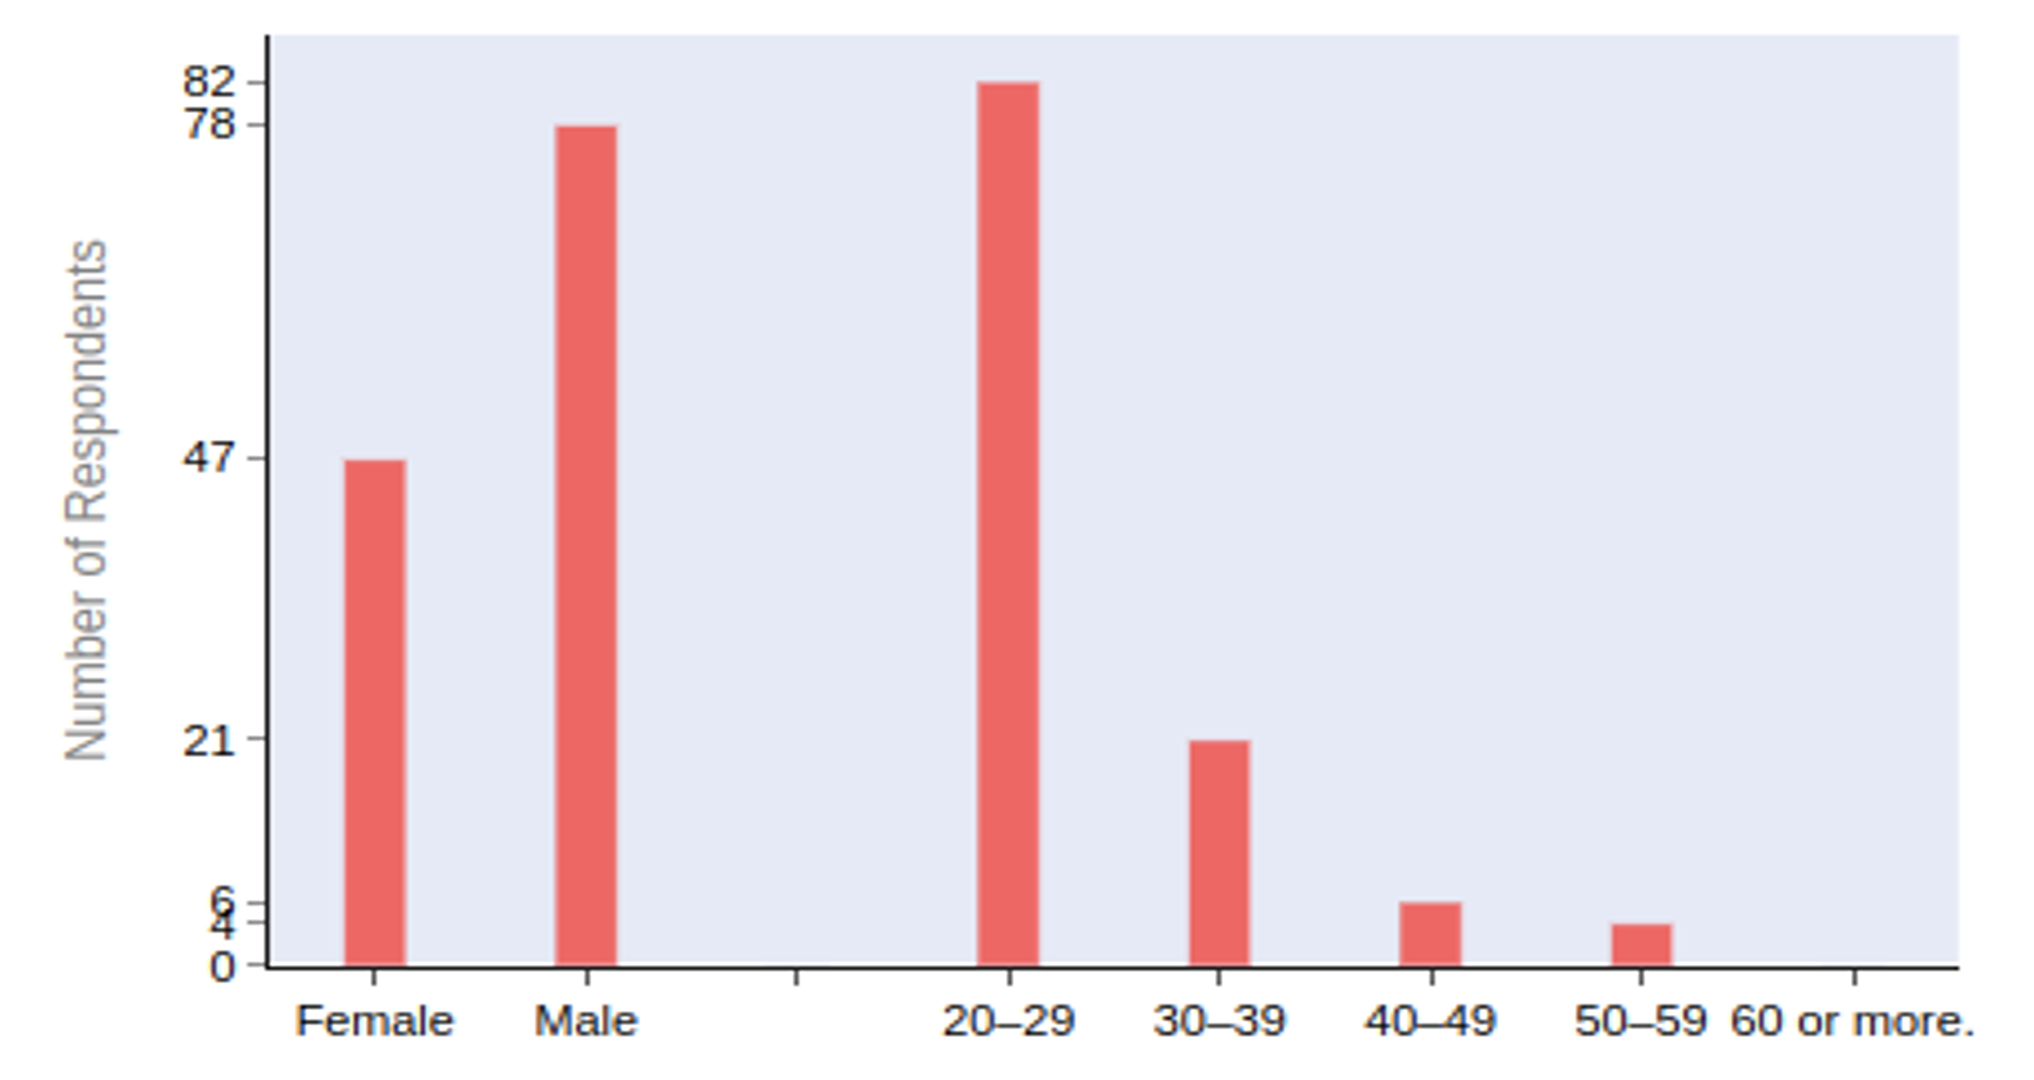
\includegraphics[width=90mm,angle=0]{demographics.png}
\end{center}
\vspace{-5mm}
\caption{Graphic depiction of the demographics of the 143 respondents who took the pilot survey}
\label{fig:demographics}       
\end{figure}

Of the 143 respondents, 78 were male, and 47 were female. This is a more balanced gender distribution than the population from which the respondents were drawn. \\

\noindent In terms of age, the majority of participants were in the 20–29 age group, followed by a smaller number in the 30–39 range. Very few respondents were aged 40–49, 50–59, or 60 and older. Despite this, the data collected represents a range of demographic groups, as shown in Figure \ref{fig:demographics}.

\subsection{Data Analysis Techniques}
%===============================================================
\label{section:data_analysis}

Significant effort was expended in performing  comprehensive data analysis to build the cultural knowledge base. This involved cleaning and organizing the collected data to ensure accuracy and consistency, and then identifying prevalent consensus answers to each question. Both qualitative and quantitative analysis methods were employed to identify key cultural elements and patterns within the responses. 

\begin{figure}[t]
\begin{center}
%\vspace{-5mm}
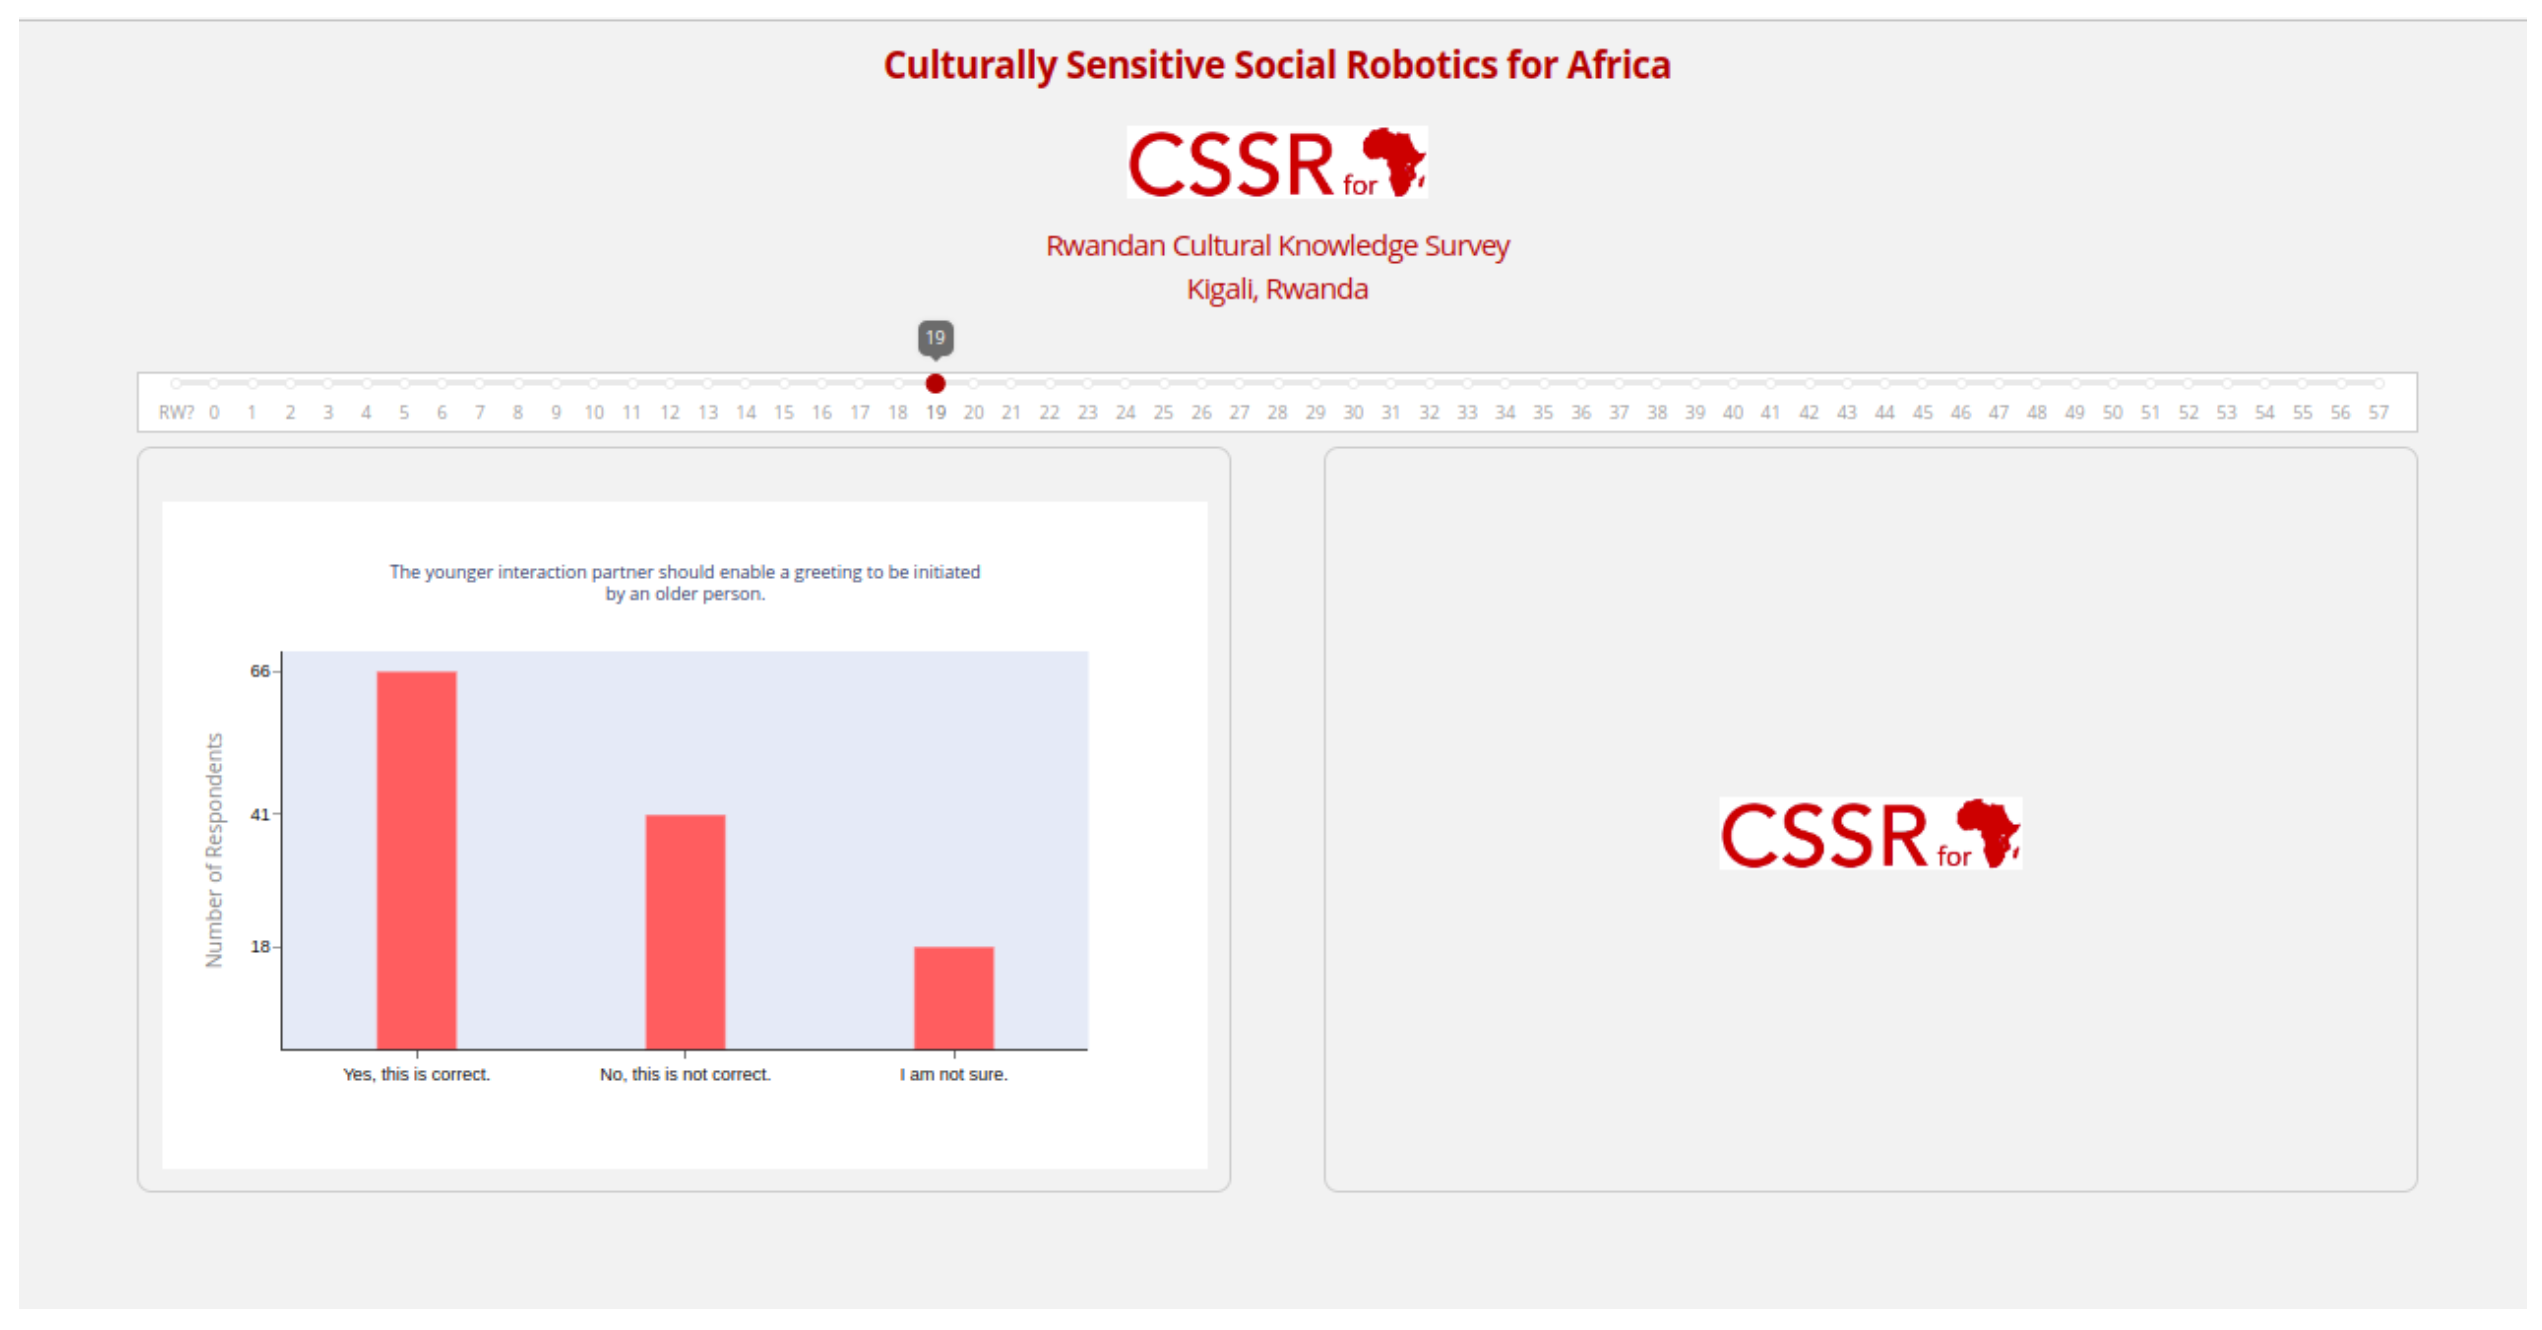
\includegraphics[width=120mm,angle=0]{dashboard1.png}
\end{center}
\vspace{-5mm}
\caption{The dashboard used to visualize the responses to each question.}
\label{fig:dashboard1}       
\end{figure}

\begin{figure}[tb]
\begin{center}
%\vspace{-5mm}
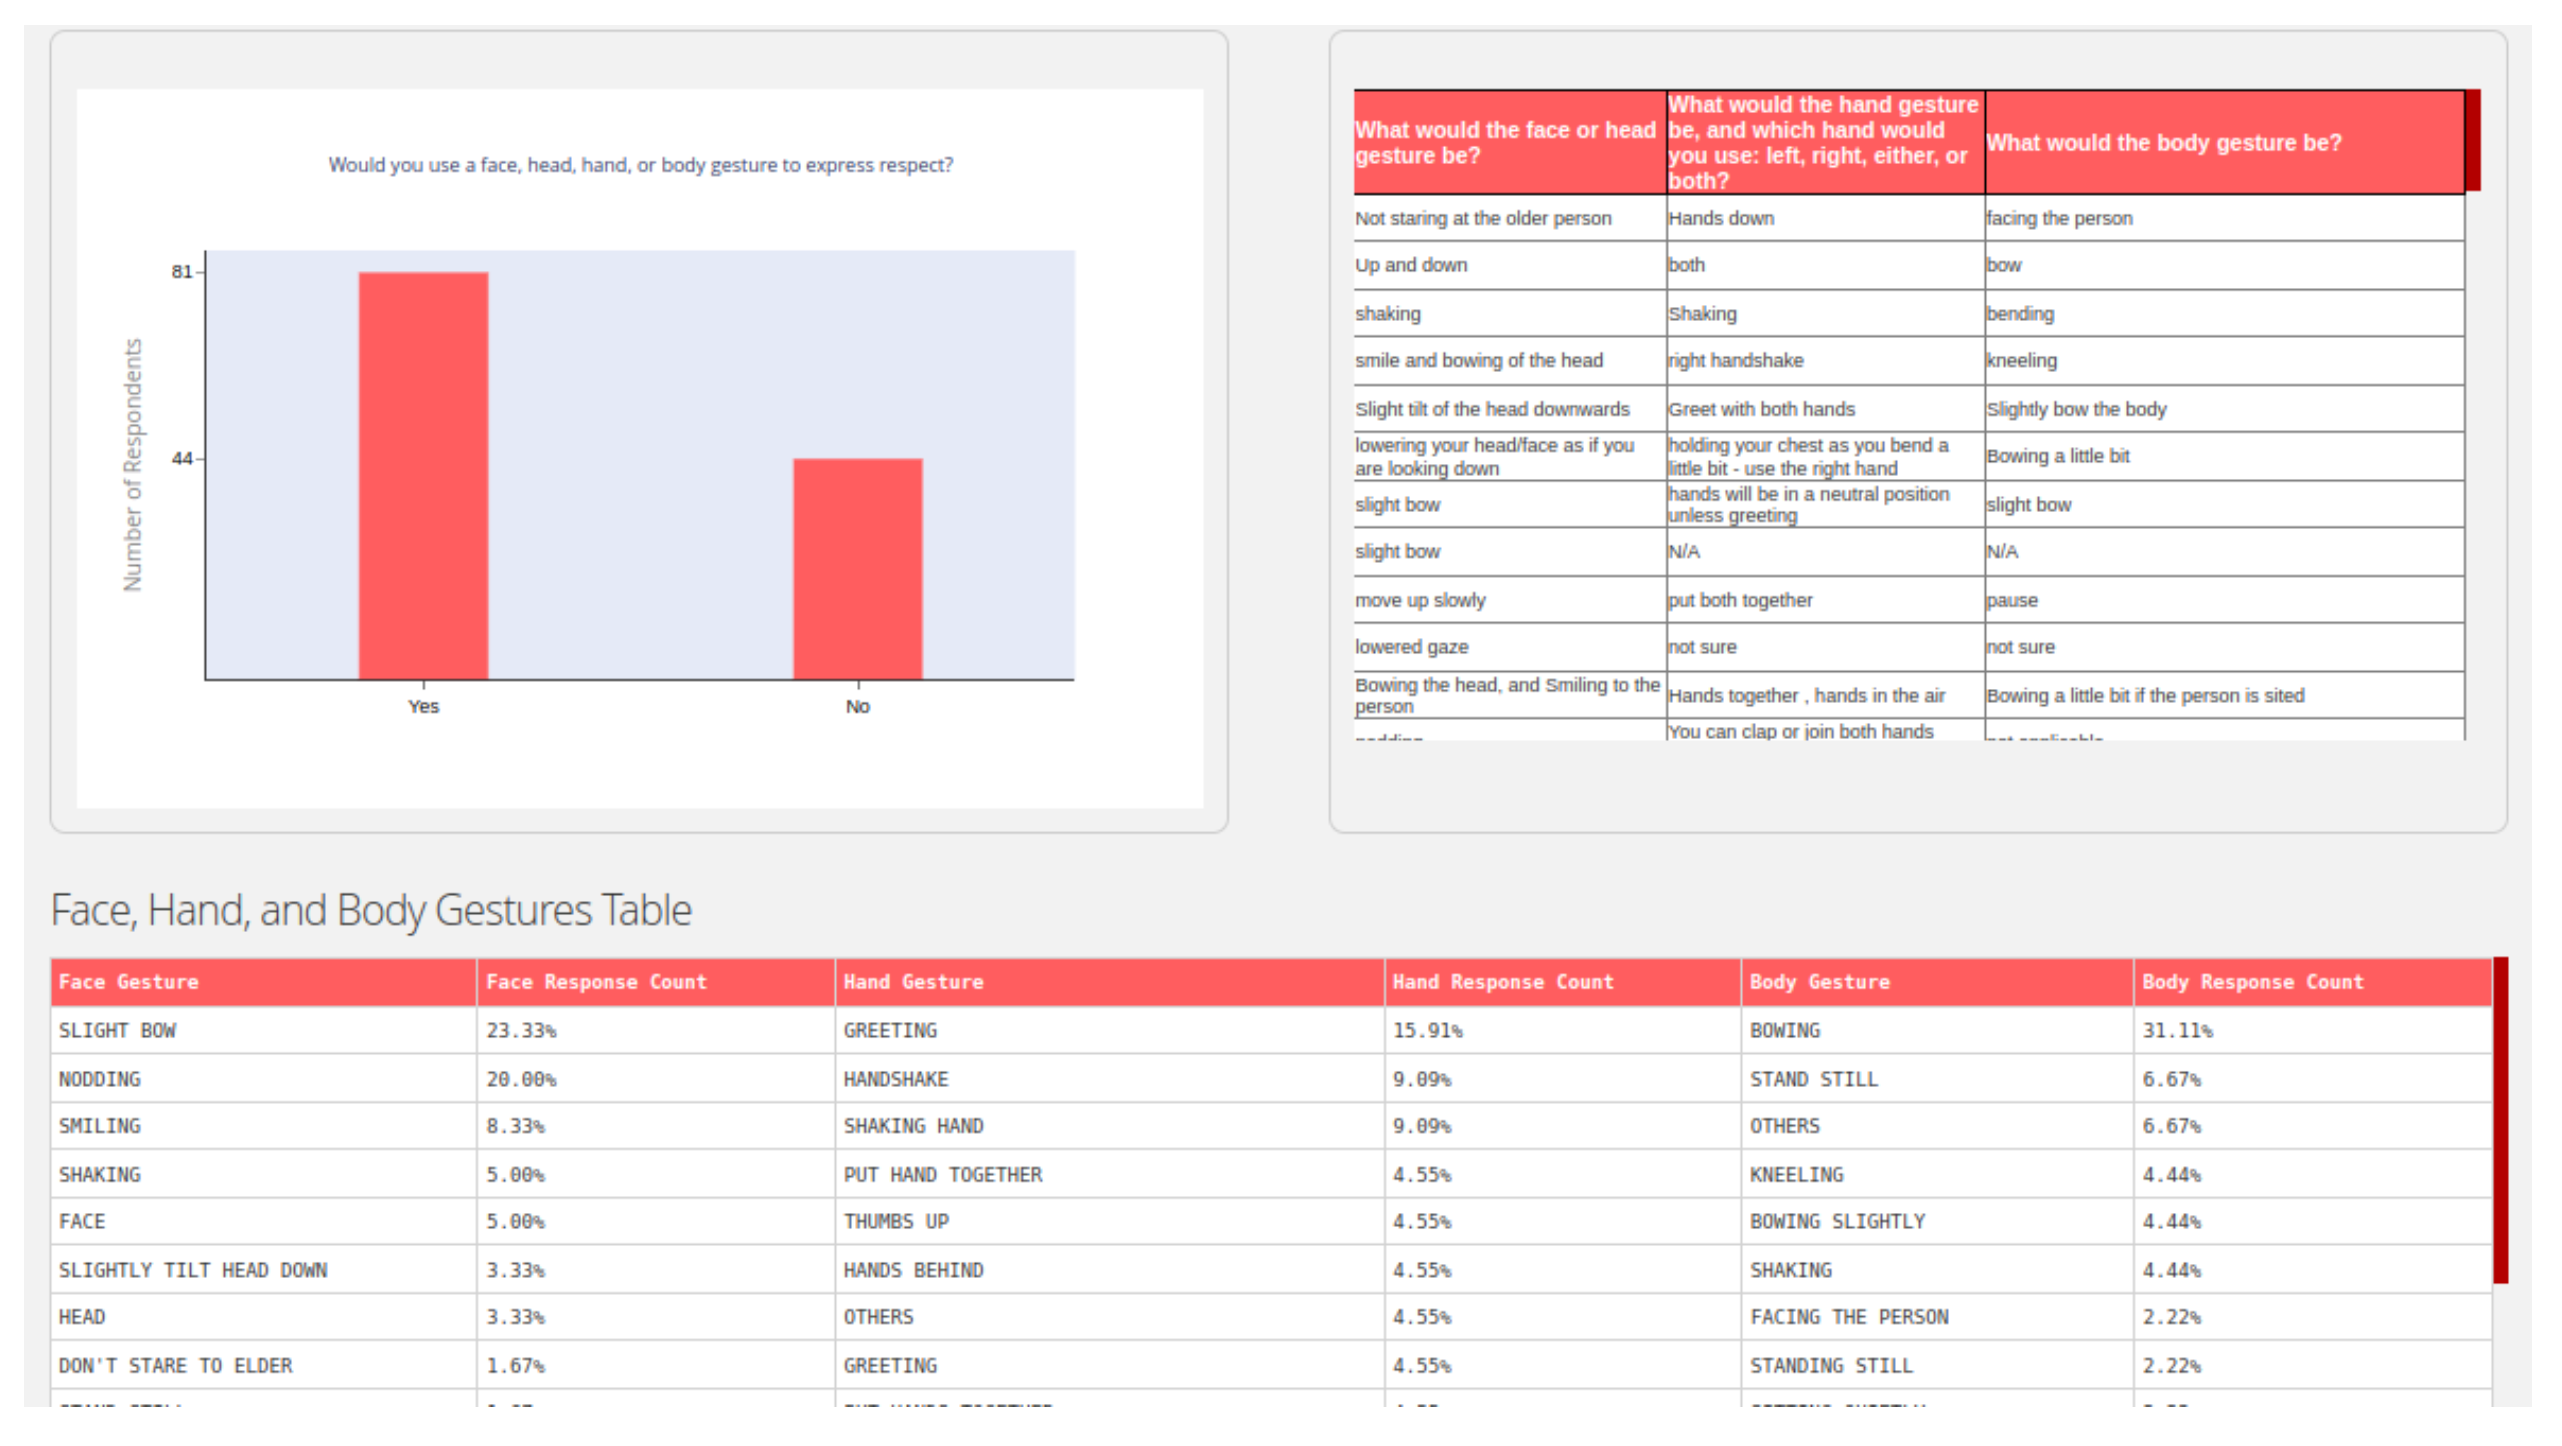
\includegraphics[width=120mm,angle=0]{dashboard2.png}
\end{center}
\vspace{-5mm}
\caption{A detailed view of dashboard used to visualize the responses to each question.}
\label{fig:dashboard2}       
\end{figure}

\begin{figure}[tb]
\begin{center}
%\vspace{-5mm}
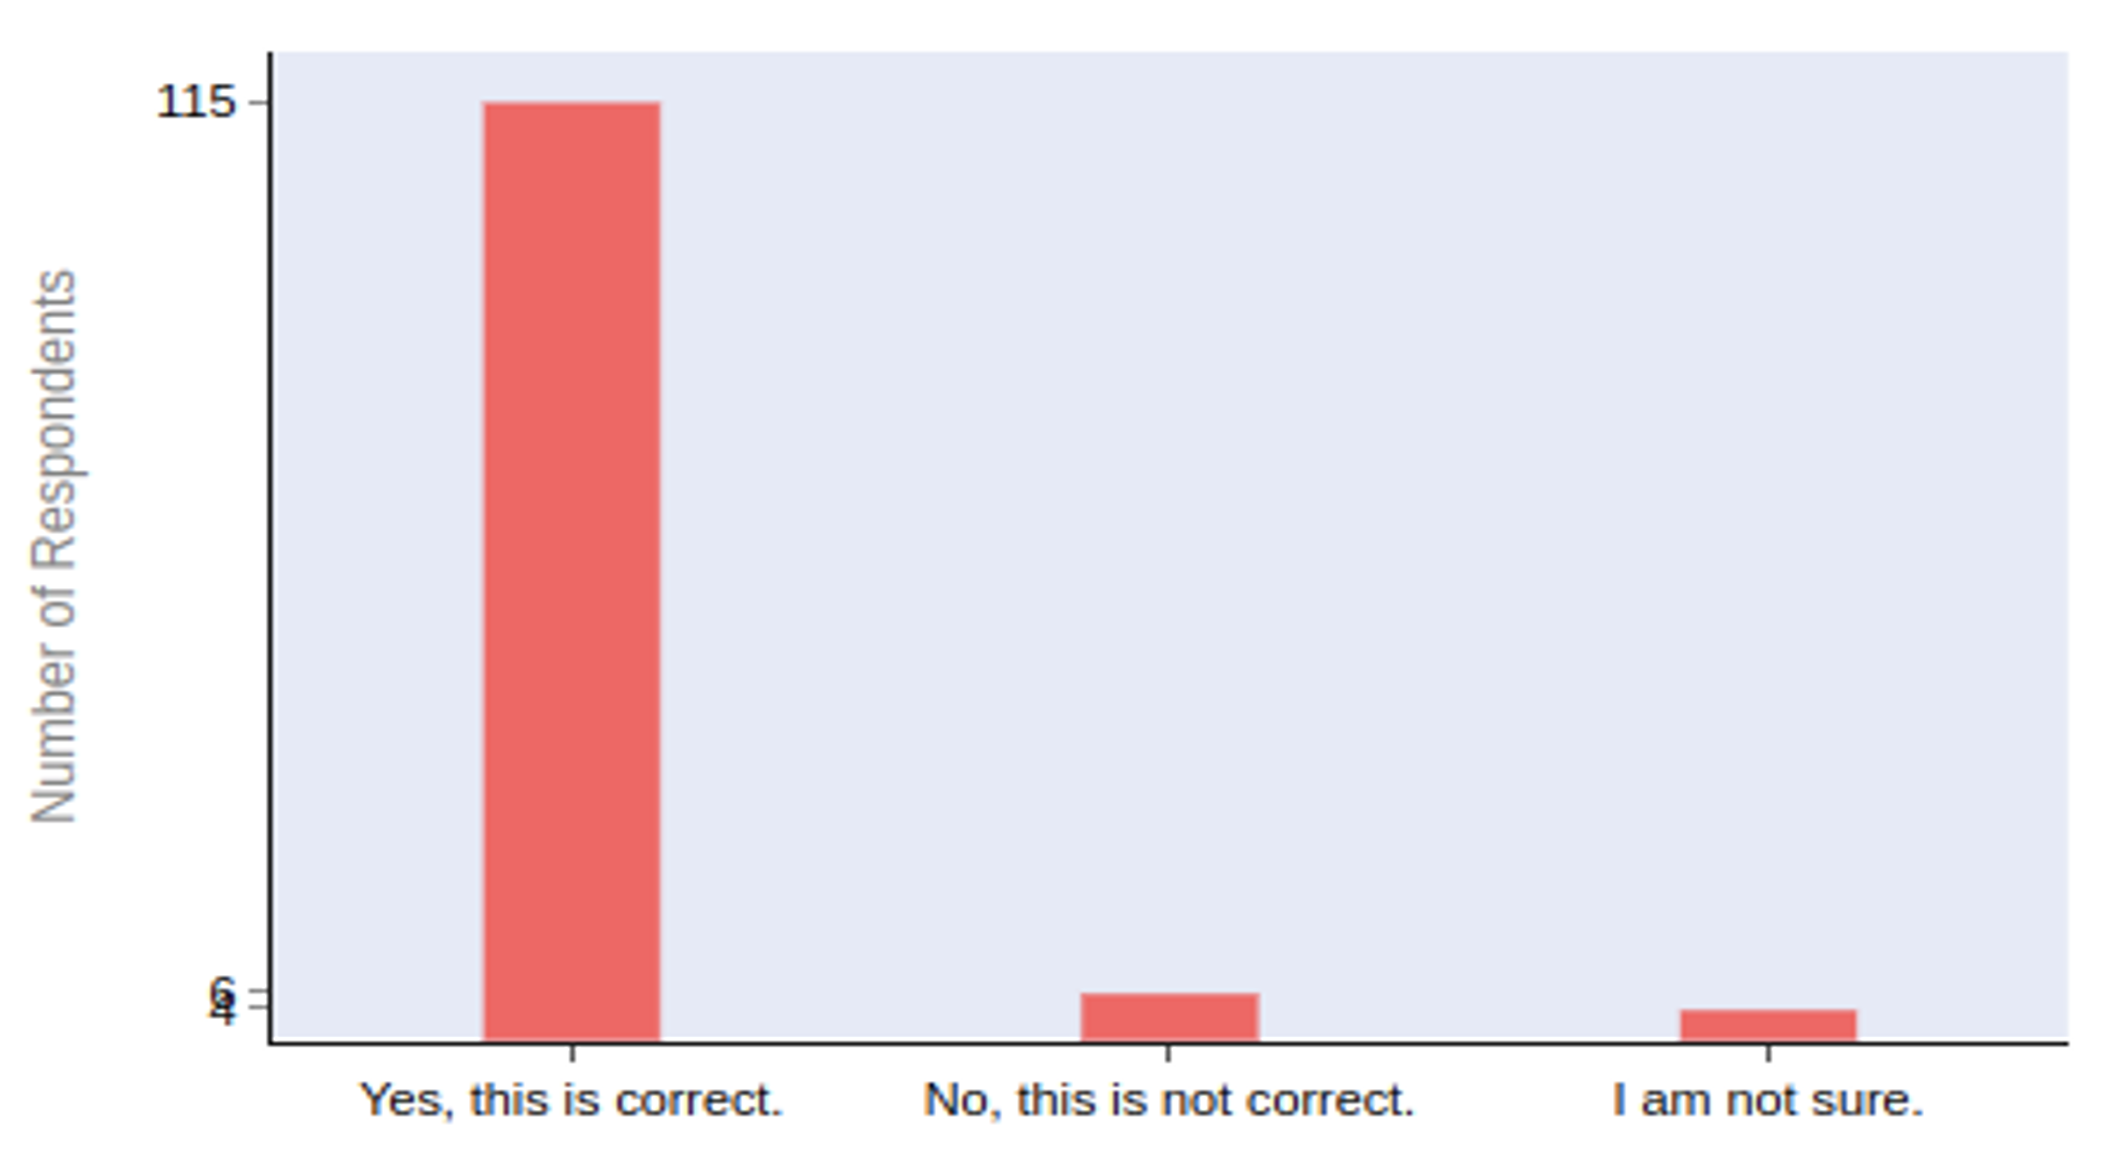
\includegraphics[width=100mm,angle=0]{consensus1.png}
\end{center}
\vspace{-5mm}
\caption{A summary of the responses for Question 2-26 One should not walk between two or more people who are conversing because it is considered rude to do so.}
\label{fig:consensus1}       
\end{figure}


\begin{figure}[tb]
\begin{center}
%\vspace{-5mm}
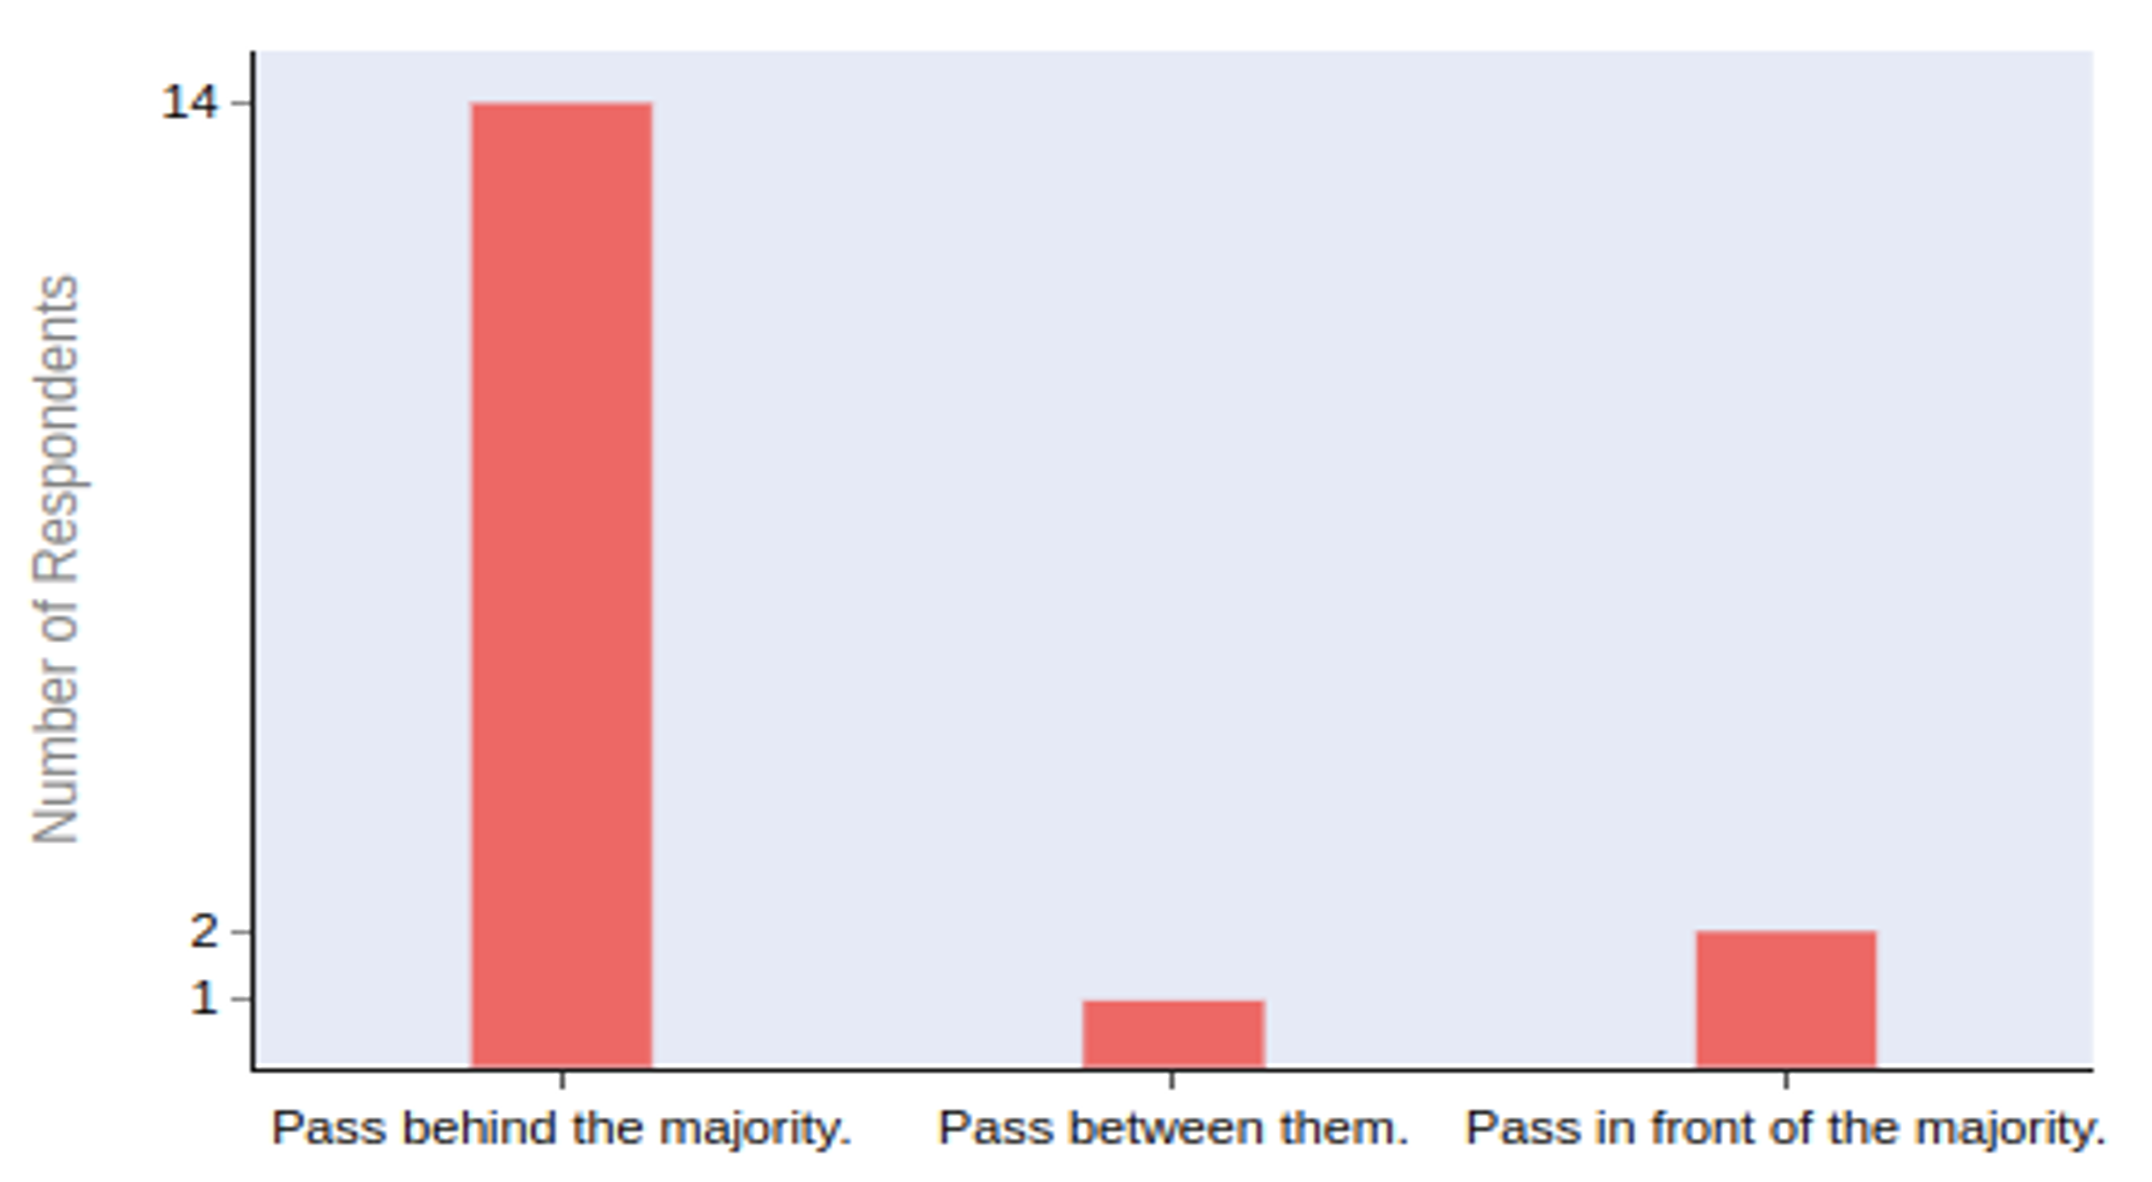
\includegraphics[width=100mm,angle=0]{consensus2.png}
\end{center}
\vspace{-5mm}
\caption{A summary of the responses for Question 3-3 How should you pass a group of two or more people?}
\label{fig:consensus2}       
\end{figure}

\noindent The data cleaning phase was carried out in two stages, an initial scan by three members of the team to identify questions for the answers were clearly equivocal, and a workshop involving ten members of the team to identify consensus answers.  In the first stage, two questions were identified --- 3.28 and 3-30 --- and they were excluded from further consideration.  In the second stage, the answers to each question were displayed and the workshop participants voted to decided on the consensus answer, if one existed.  To visualize survey responses, a dashboard was developed using Dash, a Python web framework built on Plotly that specializes in creating interactive data visualization applications. This dashboard displays all survey questions and allows users to interact with the data using a slider bar to select the question and responses for analysis. The data is presented using bar charts and tables, as illustrated in Figures \ref{fig:dashboard1} and \ref{fig:dashboard2}. This visualization framework improved accessibility and simplified the analysis of survey results. Examples of the histogram of answers to two questions are shown in Figures \ref{fig:consensus1} and \ref{fig:consensus2}.   No consensus was found for three questions ---  2-4, 2-5, and 2-8  --- and these were also excluded from futher consideration.\\

\noindent The results of this  analysis, described in Section \ref{section:knowledge},  forms the foundation for  a detailed cultural knowledge base, which will be used to guide the behavior of a Pepper social robot.
 



\clearpage

\section{Survey Results: Rwandan Cultural Knowledge for Respectful Interaction}
%===============================================================
\label{section:knowledge}


Tables \ref{table:AllAnswers2}  and \ref{table:AllAnswers3} presents the consensus answers to the subset of fifty-seven questions in the cultural knowledge survey questionnaire in Appendices I and II, after having removed the questions for which no consensus could be identified. These capture the behaviors, activities, actions, and motions that are considered polite and respectful when interacting with people in Rwanda.\\~\\

\begin{table}[H]
\begin{center}
\vspace{-5mm}
\begin{tabularx}{\linewidth}{|l|X|}
\hline \hline
 {\small {\bf Question}}  & {\small {\bf Consensus Cultural Knowledge}}\\
\hline
 {\small 2-1 } & {\small To show respect, one should lower gaze when greeting someone older.}\\
 {\small 2-2 } & {\small One should suspend work or movements and pay attention when addressed.}\\
 {\small 2-3 } & {\small One should keep intermittent eye contact; lack of eye contact depicts disrespect as it shows divided
attention during the interaction}\\
{\small 2-6 }  & {\small One should use an open palm of the hand to point to people and objects.}\\
{\small 2-7 }  & {\small One should not point an upward facing palm of the hand at someone.}\\
{\small 2-9 }  & {\small To show respect, one should bow slightly when greeting someone older.}\\
{\small 2-10 } & {\small To show respect, one should raise both hands when greeting.}\\
{\small 2-11 } & {\small One should not wave at someone from a distance; one should move towards them to greet them}\\
{\small 2-12 } & {\small One should not use the left hand to hand something to someone}\\
{\small 2-13 } & {\small To show respect, one should hand over and accept gifts with two hands and do so from the front,
facing the recipient}\\
{\small 2-14 } & {\small To show respect, one should shake hands with the right hand and use the left arm to support the
right forearm when doing so.}\\
{\small 2-15 } & {\small An appreciation of rhythmic sound and movement is valued.}\\
{\small 2-16 } & {\small To show respect, one should bow slightly and lower gaze when greeting someone older}\\
{\small 2-17 } & {\small The younger interaction partner should bow when greeting an older person or when rendering a
service}\\
{\small 2-18 } & {\small All interactions should begin with a courteous greeting.}\\
{\small 2-19 } & {\small The younger interaction partner should enable a greeting to be initiated by an older person.}\\
{\small 2-20 } & {\small It is respectful to use local languages and they should be used for verbal interaction when possible.}\\
{\small 2-21 } & {\small One should use formal titles when addressing someone.}\\
{\small 2-22 } & {\small One should engage in a preamble before getting to the point, as being too forward may be regarded as disrespectful.}\\
{\small 2-23 } & {\small One should not interrupt or talk over someone when they are speaking.}\\
{\small 2-24 } & {\small One should not talk loudly to an older person}\\
{\small 2-25 } & {\small Behaviours should focus on fostering social connections and relationships; they should not be
purely functional.}\\
{\small 2-26 } & {\small One should not walk between two or more people who are conversing because it is considered
rude to do so.}\\
{\small 2-27 } & {\small One should not walk far ahead of an older person, unless leading the person (in which case, one
should walk slightly to the side).}\\
\hline \hline
\end{tabularx}
\end{center}
\vspace{-5mm}
\caption{ Consensus answers to the subset of the twenty-seven questions in Part 2 of the cultural knowledge survey questionnaire in Appendices I and  II. Answers to questions 2-4, 2-5, and 2-8 are not listed as no consensus could be identified.}
\label{table:AllAnswers2}
\end{table}
%%%%%%%%%%%%%%%%%%%%%%%%%%%%%%%%%%%%%%%%%%%%%%%%%%%%%%%%%%%
\newpage
\begin{table}[H]
\begin{center}
\vspace{-10mm}
\begin{tabularx}{\linewidth}{|l|X|}
\hline \hline
 {\small {\bf }}  & {\small {\bf Consensus Cultural Knowledge}}\\
\hline
{\small 3-1 }  & {\small One should maintain a distance of one meter or less when passing someone.}\\

{\small 3-2 }  & {\small One should say 'Hello' or 'Muraho' when acknowledging someone while passing them.}\\

{\small 3-3 }  & {\small One should pass behind a group of two or more people.}\\

{\small 3-4 }  & {\small One should position themselves beside someone older when showing them the way.}\\

{\small 3-5 }  & {\small One should position themselves beside someone of the same age when showing them the way.}\\

{\small 3-6 }  & {\small One should position themselves beside someone younger when showing them the way.}\\

{\small 3-7--3-9 } & {\small The preferred way to address someone, whether they are older, younger, or the same age, and whom you haven't met before, is by saying 'Muraho' or 'Hello'.}\\

{\small 3-10 }  & {\small When asked a question, respondents should pause for a few seconds before answering.}\\

{\small 3-11 }  & {\small In turn-based conversations, participants can raise their right hand to signal their desire to speak.}\\

{\small 3-12 }  & {\small When explaining something to someone, you should direct your gaze equally between the person and the object.}\\

{\small 3-13 }  & {\small When explaining something to someone, you should make eye contact often.}\\

{\small 3-14 }  & {\small You should make eye contact more often when explaining something to someone older than you.}\\

{\small 3-15 }  & {\small You should make eye contact more often when explaining something to someone younger than you.}\\

{\small 3-16 }  & {\small When someone is explaining something to you, you should direct your gaze equally between the person and the object.}\\

{\small 3-17 } & {\small When someone is explaining something to you, you should make eye contact often.}\\

{\small 3-18 } & {\small If someone is explaining something to you and they are older than you, you should make eye contact more often.}\\

{\small 3-19 } & {\small If someone is explaining something to you and they are younger than you, you should make eye contact more often.}\\

{\small 3-20 } & {\small To draw someone's attention to something, use a head-nodding gesture while looking at the object.}\\

{\small 3-21 } & {\small To express gratitude, common gestures include nodding, smiling, and bowing the head, using hand gestures like a thumbs up or clasped hands, and slight bowing of the body.}\\

{\small 3-22 } & {\small To express agreement, common gestures include nodding the head and giving a thumbs up with the right hand.}\\

{\small 3-23 } & {\small To show respect, common gestures include a slight bow of the head, a greeting or handshake using the right hand supported by the left, and bowing, which is the most frequent body gesture.}\\

{\small 3-24 } & {\small To express friendliness, people commonly use facial gestures like smiling, hand gestures such as a handshake using both hands or the right hand, and body gestures like hugging.}\\

{\small 3-25 } & {\small When expressing confusion, individuals typically use facial gestures like wrinkling or frowning the brow or tilting the head, hand gestures such as raising both hands or the right hand, and body movements that vary according to the situation.}\\

{\small 3-26 } & {\small When expressing comprehension, individuals typically use head gestures, such as nodding, hand gestures like a right-hand thumbs-up, and body gestures that vary by situation.} \\

{\small 3-27 } & {\small When expressing interest, nodding and smiling are the most common gestures, while hand gestures such as giving a thumbs up with the right hand and body gestures like facing someone are used less frequently.} \\

{\small 3-29 } & {\small One should use body and hand gestures while speaking to someone, which depends on the situation. The most recommended gestures are slight body movement and slightly moving both hands.} \\
\hline \hline
\end{tabularx}
\end{center}
\vspace{-5mm}
\caption{ Consensus answers to the subset of the thirty questions in Part 3 of the cultural knowledge survey questionnaire in Appendices I and II. Answers to questions 3-28 and 3-30 are not listed as no consensus could be identified.}
\label{table:AllAnswers3}
\end{table}


\section{Conclusion}
%===============================================================
 \label{section:conclusion}

This study represents an esential  step in developing culturally sensitive social robotics for Rwanda and South Africa. The CSSR4Africa project has successfully piloted a survey at Carnegie Mellon University Africa, gathering 143 responses   that provide valuable insights into Rwandan cultural norms. The next phase involves expanding data collection in Rwanda and initiating similar studies in South Africa. Detailed analysis of the results will lead to the development of a comprehensive cultural knowledge database, which will inform the creation of a detailed cultural knowledge ontology. This ontology will ensure that social robots align with local norms. By incorporating these cultural insights, the CSSR4Africa project aims to enhance the acceptance and effectiveness of social robots in Rwanda and South Africa, promoting their successful integration in diverse African settings.


\newpage

\section*{Appendix I: Cultural Knowledge  Survey  Questionnaire  (English)}
%===============================================================
\addcontentsline{toc}{section}{Appendix I: Cultural Knowledge  Survey Questionnaire  (English) }
 
\subsection*{Respectful Interaction}
In daily life, people interact with one another in several ways. They interact verbally using speech and they interact non-verbally using body language, e.g, by gesturing with their hands, arms, shoulders, faces, lips, eyes, and eyebrows.  During such social interaction, they often position their bodies in certain ways.  It is highly desirable that all interaction between people be conducted in a respectful manner by being aware of social and cultural norms and expectations. 

\subsection*{Goal of the Survey}
This survey aims to answer the following two questions: ``How do you behave respectfully  when interacting with people in Rwanda and how should you not behave?''   

\subsection*{Purpose of the Survey}
The knowledge that is gathered in this survey will be used to equip social robots with cultural knowledge that will allow them to interact respectfully and politely with people  using non-verbal,  verbal, and spatial modes of behaviour.

\subsection*{Structure of the Questionnaire}
The questionnaire has three parts. 

In Part 1, we ask you to provide some information about yourself.  This information will be kept in strict confidence and it is only used to check that the survey is balanced in terms of age, gender, cultural heritage, and nationality. 

In Part 2, we will ask you whether  you consider cultural knowledge we have gathered in previous surveys\footnote{We canvassed the views of twenty-three people from eight countries in Africa to  collect this cultural knowledge.} to be correct or not. The focus of these surveys was on human-robot interaction, derived from human-human interaction, and so the social settings reflects situations where one might encounter a social robot, e.g., hospitals, airports, exhibitions, shopping malls, and offices.

In Part 3, we  ask you to answer several questions to help us identify different forms of culturally sensitive, respectful behaviours --- movements, actions, or activities --- and disrespectful behaviours.

\newpage
\subsection*{Part 1: Demographic Information}
%==============================================================================
\label{section:demographics}

%%\Qitem{ \Qq{What is your name}: \hskip0.4cm \Qline{4cm} }

\Qitem{\Qq{What age are you?} \Qtab{3.51cm}{

%%\QO{} Under 20 \hskip0.2cm 

\QO{} 20--29 \hskip0.2cm \QO{} 30--39 \hskip0.2cm \QO{} 40--49 \hskip0.2cm \QO{} 50--59 \hskip0.2cm \QO{} 60 or more.}}

%%\Qitem{ \Qq{What gender are you?} \hskip0.05cm \QO{} Female \hskip0.5cm \QO{} Male}

\Qitem{ \Qq{Which are you?} \hskip0.05cm \QO{} Female \hskip0.25cm \QO{} Male}

%%\Qitem{ \Qq{What is your cultural heritage?} \hskip0.26cm \Qline{5cm} }
 
%%\Qitem{ \Qq{What is your nationality?} \hskip1.11 cm \Qline{5cm} }
 
\newpage

\subsection*{Part 2: Existing Cultural Knowledge}
%==============================================================================

Consider the following statements and select the option to indicate whether or agree with it or not.

\setcounter{itemnummer}{0}

% Non-verbal Interaction.
%% Gaze.
%%% Focus of attention.
%%%%  Target.
%%%%  Duration.

\Qitem{ \Qq{To show respect, one should lower gaze when greeting someone older.}
\begin{Qlist}
\item Yes, this is correct.
\item No, this is not correct.
\item I am not sure.
\end{Qlist}
}

\Qitem{ \Qq{One should suspend work or movements and pay attention when addressed.}
\begin{Qlist}
\item Yes, this is correct.
\item No, this is not correct.
\item I am not sure.
\end{Qlist}
}

%%% Eye Contact.
%%%%  Relative Age of Interaction Partner.
%%%%  Duration.


\Qitem{ \Qq{One should keep intermittent eye contact; lack of eye contact depicts disrespect as it shows divided attention during the interaction. }
\begin{Qlist}
\item Yes, this is correct.
\item No, this is not correct.
\item I am not sure.
\end{Qlist}
}

\Qitem{ \Qq{One should not make persistent eye contact with an older person. }
\begin{Qlist}
\item Yes, this is correct.
\item No, this is not correct.
\item I am not sure.
\end{Qlist}
}

\Qitem{ \Qq{One should not make eye contact when being corrected by someone. }
\begin{Qlist}
\item Yes, this is correct.
\item No, this is not correct.
\item I am not sure.
\end{Qlist}
}

%% face or head Gesture.
%%% Lips.
%%%%  Shape.
%%%%  Intensity.
%%% Eyebrow.
%%%%  Shape.
%%%%  Intensity.
%% Hand Gesture.
%%%%  Shape.
%%%%  Duration.
%%% Deictic (Indicating).
%%%%  Shape.
%%%%  Meaning.

\Qitem{ \Qq{One should use an open palm of the hand to point to people and objects.}
\begin{Qlist}
\item Yes, this is correct.
\item No, this is not correct.
\item I am not sure.
\end{Qlist}
}


\Qitem{ \Qq{One should not point an upward facing palm of the hand at someone.}
\begin{Qlist}
\item Yes, this is correct.
\item No, this is not correct.
\item I am not sure.
\end{Qlist}
}


\Qitem{ \Qq{One should not use the left hand to point to anything.}
\begin{Qlist}
\item Yes, this is correct.
\item No, this is not correct.
\item I am not sure.
\end{Qlist}
}

\newpage

%%% Iconic.


%%% Symbolic.
%%%%  Shape.
%%%%  Meaning.


\Qitem{ \Qq{To show respect, one should bow slightly when greeting someone older.}
\begin{Qlist}
\item Yes, this is correct.
\item No, this is not correct.
\item I am not sure.
\end{Qlist}
}

\Qitem{ \Qq{To show respect, one should raise both hands when greeting.}
\begin{Qlist}
\item Yes, this is correct.
\item No, this is not correct.
\item I am not sure.
\end{Qlist}
}

\Qitem{ \Qq{One should not wave at someone from a distance; one should move towards them to greet them.}
\begin{Qlist}
\item Yes, this is correct.
\item No, this is not correct.
\item I am not sure.
\end{Qlist}
}


\Qitem{ \Qq{One should not use the left hand to hand something to someone.}
\begin{Qlist}
\item Yes, this is correct.
\item No, this is not correct.
\item I am not sure.
\end{Qlist}
}


\Qitem{ \Qq{To show respect, one should hand over and accept gifts with two hands and do so from the front, facing the recipient.}
\begin{Qlist}
\item Yes, this is correct.
\item No, this is not correct.
\item I am not sure.
\end{Qlist}
}

\Qitem{ \Qq{To show respect, one should shake hands with the right hand and use the left arm to support the right forearm when doing so. }
\begin{Qlist}
\item Yes, this is correct.
\item No, this is not correct.
\item I am not sure.
\end{Qlist}
}

 

%%% Beat.
%%%%  Shape.
%%%%  Intensity.

\Qitem{ \Qq{An appreciation of rhythmic sound and movement is valued.   }
\begin{Qlist}
\item Yes, this is correct.
\item No, this is not correct.
\item I am not sure.
\end{Qlist}
}


%% Body Gesture.
%%% Shoulder.
%%%%  Dropped / Raised.
%%%%  Intensity.
%%%%  Speed.

%%% Bow.
%%%%  Extent.
%%%%  Speed.


\Qitem{ \Qq{To show respect, one should bow slightly and lower gaze when greeting someone older.}
\begin{Qlist}
\item Yes, this is correct.
\item No, this is not correct.
\item I am not sure.
\end{Qlist}
}

\newpage

\Qitem{ \Qq{The younger interaction partner should bow when greeting an older person or when rendering a service.}
\begin{Qlist}
\item Yes, this is correct.
\item No, this is not correct.
\item I am not sure.
\end{Qlist}
}



%Verbal Interaction.
%%Words.
%%% Loudness.
%%% Speed.
%%% Intonation.
%%% Stress.
%%% Rhythm.



\Qitem{ \Qq{All interactions should begin with a courteous greeting.}
\begin{Qlist}
\item Yes, this is correct.
\item No, this is not correct.
\item I am not sure.
\end{Qlist}
}

\Qitem{ \Qq{The younger interaction partner should enable a greeting to be initiated by an older person.}
\begin{Qlist}
\item Yes, this is correct.
\item No, this is not correct.
\item I am not sure.
\end{Qlist}
}

\Qitem{ \Qq{It is respectful to use local languages and they should be used for verbal interaction when possible. }
\begin{Qlist}
\item Yes, this is correct.
\item No, this is not correct.
\item I am not sure.
\end{Qlist}
}

\Qitem{ \Qq{One should use formal titles when addressing someone.}
\begin{Qlist}
\item Yes, this is correct.
\item No, this is not correct.
\item I am not sure.
\end{Qlist}
}

\Qitem{ \Qq{One should engage in a preamble before getting to the point, as being too forward may be regarded as disrespectful. }
\begin{Qlist}
\item Yes, this is correct.
\item No, this is not correct.
\item I am not sure.
\end{Qlist}
}

 

\Qitem{ \Qq{One should not interrupt or talk over someone when they are speaking. }
\begin{Qlist}
\item Yes, this is correct.
\item No, this is not correct.
\item I am not sure.
\end{Qlist}
}

\Qitem{ \Qq{One should not talk loudly to an older person.}
\begin{Qlist}
\item Yes, this is correct.
\item No, this is not correct.
\item I am not sure.
\end{Qlist}
}


\newpage


\Qitem{ \Qq{Behaviours should focus on fostering social connections and relationships; they should not be purely functional. }
\begin{Qlist}
\item Yes, this is correct.
\item No, this is not correct.
\item I am not sure.
\end{Qlist}
}

%% Filler Sound.
%%% Frequency
%% Pause.
%%% Frequency


% Spatial Interaction.

%%  Standing.
%%%  Relative Distance.
%%%  Relative Orientation.


%% Approaching.
%%%  Relative Distance.
%%%  Relative Orientation.
%%%  Speed.


%% Passing.
%%%  Single Person.
%%%% Relative Distance.
%%%% Speed.

%%%  Group of People.
%%%% Relative Distance.
%%%% Speed.


\Qitem{ \Qq{One should not walk between two or more people who are conversing because it is considered rude to do so. }
\begin{Qlist}
\item Yes, this is correct.
\item No, this is not correct.
\item I am not sure.
\end{Qlist}
}

%% Accompanying.
%%%  Relative Distance (+/-).
 
\Qitem{ \Qq{One should not walk far ahead of an older person, unless leading the person (in which case, one should walk slightly to the side). }
\begin{Qlist}
\item Yes, this is correct.
\item No, this is not correct.
\item I am not sure.
\end{Qlist}
}
  
\newpage

\subsection*{Part 3: New Cultural Knowledge}
%=============================================================================

\setcounter{itemnummer}{0}

% Spatial Interaction.
%====================

%%  Standing.
%--------------------
%%%  Relative Distance.
%%%  Relative Orientation.


%% Approaching.
%--------------------
%%%  Relative Distance.
%%%  Relative Orientation.
%%%  Speed.

%% Passing.
%--------------------

%%%  Single Person.
%%%% Relative Distance.
%%%% Speed.

\Qitem{ \Qq{What distance should you keep when passing someone?}
\begin{Qlist}
\item Less than 1 m.
\item 1 -- 2 m.
\item More than 2 m.
\end{Qlist}
}


\Qitem{ \Qq{How should you acknowledge someone when passing them?}
\begin{Qlist}
\item No acknowledgement.
\item Raise eyebrows slightly.
\item Nod head.
\item Say hello.
\item Other. Please specify: \Qline{5cm} 
\end{Qlist}
}


%%%  Group of People.
%%%% Relative Distance.
%%%% Speed.


\Qitem{ \Qq{How should you pass a group of two or more people?}
\begin{Qlist}
\item Pass behind them.
\item Pass between them.
\item Pass in front of them.
\item Pass beside them.
\end{Qlist}
}

%% Accompanying.
%--------------------
%%%  Relative Distance (+/-).

 \Qitem{ \Qq{When showing someone {\em older} than you the way, where should you position yourself?}
\begin{Qlist}
\item Far in front of them.
\item A little in front of them.
\item Beside them.
\item A little behind them.
\end{Qlist}
}

 \Qitem{ \Qq{When showing someone {\em the same age} as you the way, where should you position yourself?}
\begin{Qlist}
\item Far in front of them.
\item A little in front of them.
\item Beside them.
\item A little behind them.
\end{Qlist}
}

 \Qitem{ \Qq{When showing someone {\em younger} than you the way, where should you position yourself?}
\begin{Qlist}
\item Far in front of them.
\item A little in front of them.
\item Beside them.
\item A little behind them.
\end{Qlist}
}

\newpage

%Verbal Interaction.
%===================

%%Words.
%--------------------
%%% Loudness.
%%% Speed.
%%% Intonation.
%%% Stress.
%%% Rhythm.


\Qitem{ \Qq{How should you address someone who is {\em older} than you and who you haven't met before?}
\begin{Qlist}
\item First name.
\item Last name.
\item Title first name.
\item Title last name.
\item Muraho.
\item Mwaramutse or Mwiriwe
\item Other. Please specify: \Qline{5cm} 
\end{Qlist}
}
 

\Qitem{ \Qq{How should you address someone who is {\em the same age} as you and who you haven't met before?}
\begin{Qlist}
\item First name.
\item Last name.
\item Title first name.
\item Title last name.
\item Muraho.
\item Mwaramutse or Mwiriwe
\item Other. Please specify: \Qline{5cm} 
\end{Qlist}
}


\Qitem{ \Qq{How should you address someone who is {\em younger} than you and who you haven't met before?}
\begin{Qlist}
\item First name.
\item Last name.
\item Title first name.
\item Title last name.
\item Muraho.
\item Mwaramutse or Mwiriwe
\item Other. Please specify: \Qline{5cm} 
\end{Qlist}
}

\vspace{-5mm}\textcolor{black}{\Qitem{ \Qq{Should you pause before responding when someone asks you a question? If yes, for how long?}
\begin{Qlist}
\item Yes: \Qline{5cm} 
\item No.
\end{Qlist}
}
}
 

\vspace{-5mm}\textcolor{black}{\Qitem{ \Qq{In an interaction where you and someone else take turns to speak, would you signal that you want to speak? If yes, how do you do that?}
\begin{Qlist}
\item Yes: \Qline{5cm} 
\item No.
\end{Qlist}
}
}



%% Filler Sound.
%--------------------
%%% Frequency

%% Pause.
%--------------------
%%% Frequency

\newpage

% Non-verbal Interaction.
%===============

%% Gaze.
%--------------------
%%% Focus of attention.
%%%%  Target.
%%%%  Duration.



%%% Eye Contact.
%%%%  Relative Age of Interaction Partner.
%%%%  Duration.

\Qitem{ \Qq{If {\em you} are explaining something to someone, what is your primary focus of attention, i.e., where do you direct your gaze?}
\begin{Qlist}
\item The object being explained.
\item The face, eyes, or mouth of the person to whom you are explaining.
\item Mostly the object and sometimes the person.
\item Mostly the person and sometimes the object.
\item Equally the person and the object.
\end{Qlist}
}
 


\Qitem{ \Qq{If {\em you} are explaining something to someone, how often should you make eye contact?}
\begin{Qlist}
\item Never.
\item Occasionally.
\item Often.
\item Constantly.
\end{Qlist}
}

\Qitem{ \Qq{If {\em you} are explaining something to someone, how often would you make eye contact if the person was older than you?}
\begin{Qlist}
\item Less often.
\item More often.
\item No difference.
\end{Qlist}
}


\Qitem{ \Qq{If {\em you} are explaining something to someone, how often would you make eye contact if the person was younger than you?}
\begin{Qlist}
\item Less often.
\item More often.
\item No difference.
\end{Qlist}
}

\Qitem{ \Qq{If someone is explaining something to {\em you}, what is your primary focus of attention, i.e., where do you direct your gaze?}
\begin{Qlist}
\item The object being explained.
\item The face, eyes, or mouth of the person to whom you are explaining.
\item Mostly the object and sometimes the person.
\item Mostly the person and sometimes the object.
\item Equally the person and the object.
\end{Qlist}
}

\Qitem{ \Qq{If someone is explaining something to {\em you},  how often should you make eye contact?}
\begin{Qlist}
\item Never.
\item Occasionally.
\item Often.
\item Constantly.
\end{Qlist}
}
 
\newpage

\Qitem{ \Qq{If someone is explaining something to {\em you},  how often would you make eye contact if the person was older than you?}
\begin{Qlist}
\item Less often.
\item More often.
\item No difference.
\end{Qlist}
}


\Qitem{ \Qq{If someone is explaining something to {\em you},  how often would you make eye contact if the person was younger than you?}
\begin{Qlist}
\item Less often.
\item More often.
\item No difference.
\end{Qlist}
}

\Qitem{ \Qq{Would you use a face or head gesture to draw someone's attention  to something? \\If yes, what would that gesture be?}
\begin{Qlist}
\item Yes: \Qline{5cm}
\item No.
\end{Qlist}
}



%% face or head Gesture.
%--------------------
%%% Lips.
%%%%  Shape.
%%%%  Intensity.

%%% Eyebrow.
%%%%  Shape.
%%%%  Intensity.


\Qitem{ \Qq{Would you use a face, head, hand, or body gesture to express {\em gratitude}?}
\begin{Qlist}
\item Yes:
  \begin{Qlist}
      \item What would the face or head gesture be? \hspace{1mm} \Qline{5cm}
      \item What would the hand gesture be, and which hand would you use: left, right, either, or both? \hspace{1mm} \Qline{5cm} , \hspace{1mm} \Qline{3.8cm} 
      \item What would the body gesture be? \hspace{1mm} \Qline{5cm}
  \end{Qlist}
\item No.
\end{Qlist}
}



%\begin{Qlist}
%\item Yes:\\
%\Qline{8cm},\\ \Qline{8cm},\\ \Qline{8cm}
%\item No.
%\end{Qlist}
%}

\begin{comment}
%--------------------------------------------------------------------------------------------------
\Qitem{ \Qq{Would you use a face or head gesture to express {\em approval}? \\If yes, what would that gesture be?}
\begin{Qlist}
\item Yes: \Qline{5cm}  
\item No.
\end{Qlist}
}
 
\Qitem{ \Qq{Would you use a face or head gesture to express {\em surprise}? \\If yes, what would that gesture be?}
\begin{Qlist}
\item Yes: \Qline{5cm}  
\item No.
\end{Qlist}
}
 \end{comment}
%--------------------------------------------------------------------------------------------------


\Qitem{ \Qq{Would you use a face,  head, hand, or body gesture to express {\em agreement}?}
\begin{Qlist}
\item Yes:
    \begin{Qlist}
      \item What would the face or head gesture be? \hspace{1mm} \Qline{5cm}
      \item What would the hand gesture be, and which hand would you use: left, right, either, or both? \hspace{1mm} \Qline{5cm} , \hspace{1mm} \Qline{3.8cm} 
      \item What would the body gesture be? \hspace{1mm} \Qline{5cm}
  \end{Qlist}
\item No.
\end{Qlist}
}


\Qitem{ \Qq{Would you use a face,  head, hand, or body gesture to express {\em respect}?}
\begin{Qlist}
\item Yes:
    \begin{Qlist}
      \item What would the face or head gesture be? \hspace{1mm} \Qline{5cm}
      \item What would the hand gesture be, and which hand would you use: left, right, either, or both? \hspace{1mm} \Qline{5cm} , \hspace{1mm} \Qline{3.8cm} 
      \item What would the body gesture be? \hspace{1mm} \Qline{5cm}
  \end{Qlist}
\item No.
\end{Qlist}
}

\newpage 
\Qitem{ \Qq{Would you use a face,  head, hand, or body gesture to express {\em friendliness}? }
\begin{Qlist}
\item Yes: 
    \begin{Qlist}
      \item What would the face or head gesture be? \hspace{1mm} \Qline{5cm}
      \item What would the hand gesture be, and which hand would you use: left, right, either, or both? \hspace{1mm} \Qline{5cm} , \hspace{1mm} \Qline{3.8cm} 
      \item What would the body gesture be? \hspace{1mm} \Qline{5cm}
  \end{Qlist}
\item No.
\end{Qlist}
}
 
 
\begin{comment}
%--------------------------------------------------------------------------------------------------
\Qitem{ \Qq{Would you use a face or head gesture to express {\em anger}? \\If yes, what would that gesture be?}
\begin{Qlist}
\item Yes: \Qline{5cm} 
\item No.
\end{Qlist}
}
 
\Qitem{ \Qq{Would you use a face or head gesture to express {\em fear}? \\If yes, what would that gesture be?}
\begin{Qlist}
\item Yes: \Qline{5cm}  
\item No.
\end{Qlist}
}
 
\Qitem{ \Qq{Would you use a face or head gesture to express {\em happiness}? \\If yes, what would that gesture be?}
\begin{Qlist}
\item Yes: \Qline{5cm}  
\item No.
\end{Qlist}
}
 

\Qitem{ \Qq{Would you use a face or head gesture to express {\em sadness}? \\If yes, what would that gesture be?}
\begin{Qlist}
\item Yes: \Qline{5cm}  
\item No.
\end{Qlist}
}
\end{comment}
%--------------------------------------------------------------------------------------------------

\Qitem{ \Qq{Would you use a face,  head, hand, or body gesture to express {\em confusion}?}
\begin{Qlist}
\item Yes: 
    \begin{Qlist}
      \item What would the face or head gesture be? \hspace{1mm} \Qline{5cm}
      \item What would the hand gesture be, and which hand would you use: left, right, either, or both? \hspace{1mm} \Qline{5cm} , \hspace{1mm} \Qline{3.8cm} 
      \item What would the body gesture be? \hspace{1mm} \Qline{5cm}
  \end{Qlist}
\item No.
\end{Qlist}
}


\vspace{-5mm}\textcolor{black}{\Qitem{ \Qq{Would you use a face,  head, hand, or body gesture to express {\em comprehension}? }
\begin{Qlist}
\item Yes:
    \begin{Qlist}
      \item What would the face or head gesture be? \hspace{1mm} \Qline{5cm}
      \item What would the hand gesture be, and which hand would you use: left, right, either, or both? \hspace{1mm} \Qline{5cm} , \hspace{1mm} \Qline{3.8cm} 
      \item What would the body gesture be? \hspace{1mm} \Qline{5cm}
  \end{Qlist}
\item No.
\end{Qlist}
}
}
 
\vspace{-5mm}\textcolor{black}{\Qitem{ \Qq{Would you use a face,  head, hand, or body gesture to express {\em interest}?}
\begin{Qlist}
\item Yes: 
   \begin{Qlist}
      \item What would the face or head gesture be? \hspace{1mm} \Qline{5cm}
      \item What would the hand gesture be, and which hand would you use: left, right, either, or both? \hspace{1mm} \Qline{5cm} , \hspace{1mm} \Qline{3.8cm} 
      \item What would the body gesture be? \hspace{1mm} \Qline{5cm}
  \end{Qlist}
\item No.
\end{Qlist}
}
}


\Qitem{ \Qq{Is there  a face head, hand, or body gesture you should {\em not} use?}
\begin{Qlist}
\item Yes: 
    \begin{Qlist}
      \item What would the face or head gesture be? \hspace{1mm} \Qline{5cm}
      \item What would the hand gesture be, and which hand would you use: left, right, either, or both? \hspace{1mm} \Qline{5cm} , \hspace{1mm} \Qline{ 3.8cm} 
      \item What would the body gesture be? \hspace{1mm} \Qline{5cm}
  \end{Qlist}
\item No.
\end{Qlist}
}
 


%% Hand Gesture.
%--------------------
%%% Deictic (Indicating).
%%%%  Shape.
%%%%  Duration.

%%% Iconic.
%%%%  Shape.
%%%%  Meaning.

%%% Symbolic.
%%%%  Shape.
%%%%  Meaning.


\begin{comment}
%--------------------------------------------------------------------------------------------------
\Qitem{ \Qq{Would you use a hand gesture to express {\em gratitude}? \\If yes, what would that gesture be, and which hand would you use: left, right, either, or both?}
\begin{Qlist}
\item Yes: \Qline{5cm} , \hspace{1mm} \Qline{2cm} 
\item No.
\end{Qlist}
}
 
\Qitem{ \Qq{Would you use a hand gesture to express {\em approval}? \\If yes, what would that gesture be, and which hand would you use: left, right, either, or both?}
\begin{Qlist}
\item Yes: \Qline{5cm} , \hspace{1mm} \Qline{2cm} 
\item No.
\end{Qlist}
}

\newpage
 
\Qitem{ \Qq{Would you use a hand gesture to express {\em surprise}? \\If yes, what would that gesture be, and which hand would you use: left, right, either, or both?}
\begin{Qlist}
\item Yes: \Qline{5cm} , \hspace{1mm} \Qline{2cm} 
\item No.
\end{Qlist}
}



\Qitem{ \Qq{Would you use a hand gesture to express {\em agreement}? \\If yes, what would that gesture be, and which hand would you use: left, right, either, or both?}
\begin{Qlist}
\item Yes: \Qline{5cm} , \hspace{1mm} \Qline{2cm} 
\item No.
\end{Qlist}
}

 
\Qitem{ \Qq{Would you use a hand gesture to express {\em respect}? \\If yes, what would that gesture be, and which hand would you use: left, right, either, or both?}
\begin{Qlist}
\item Yes: \Qline{5cm} , \hspace{1mm} \Qline{2cm} 
\item No.
\end{Qlist}
}
 
\Qitem{ \Qq{Would you use a hand gesture to express {\em friendliness}? \\If yes, what would that gesture be, and which hand would you use: left, right, either, or both?}
\begin{Qlist}
\item Yes: \Qline{5cm} , \hspace{1mm} \Qline{2cm} 
\item No.
\end{Qlist}
}


\Qitem{ \Qq{Would you use a hand gesture to express {\em anger}? \\If yes, what would that gesture be, and which hand would you use: left, right, either, or both?}
\begin{Qlist}
\item Yes: \Qline{5cm} , \hspace{1mm} \Qline{2cm} 
\item No.
\end{Qlist}
}
 
\Qitem{ \Qq{Would you use a hand gesture to express {\em fear}? \\If yes, what would that gesture be, and which hand would you use: left, right, either, or both?}
\begin{Qlist}
\item Yes: \Qline{5cm} , \hspace{1mm} \Qline{2cm} 
\item No.
\end{Qlist}
}
 
\Qitem{ \Qq{Would you use a hand gesture to express {\em happiness}? \\If yes, what would that gesture be, and which hand would you use: left, right, either, or both?}
\begin{Qlist}
\item Yes: \Qline{5cm} , \hspace{1mm} \Qline{2cm} 
\item No.
\end{Qlist}
}

\Qitem{ \Qq{Would you use a hand gesture to express {\em sadness}? \\If yes, what would that gesture be, and which hand would you use: left, right, either, or both?}
\begin{Qlist}
\item Yes: \Qline{5cm} , \hspace{1mm} \Qline{2cm} 
\item No.
\end{Qlist}
}
 

\Qitem{ \Qq{Would you use a hand gesture to express {\em confusion}? \\If yes, what would that gesture be, and which hand would you use: left, right, either, or both?}
\begin{Qlist}
\item Yes: \Qline{5cm} , \hspace{1mm} \Qline{2cm} 
\item No.
\end{Qlist}
}

\Qitem{ \Qq{Would you use a hand gesture to express {\em comprehension}? \\If yes, what would that gesture be, and which hand would you use: left, right, either, or both?}
\begin{Qlist}
\item Yes: \Qline{5cm} , \hspace{1mm} \Qline{2cm} 
\item No.
\end{Qlist}
}

\Qitem{ \Qq{Would you use a hand gesture to express {\em interest}? \\If yes, what would that gesture be, and which hand would you use: left, right, either, or both?}
\begin{Qlist}
\item Yes: \Qline{5cm} , \hspace{1mm} \Qline{2cm} 
\item No.
\end{Qlist}
}
\end{comment}
%--------------------------------------------------------------------------------------------------

\vspace{-5mm}\textcolor{black}{\Qitem{ \Qq{Would you use a hand or body gesture while speaking to someone? }
\begin{Qlist}
\item Yes: 
    \begin{Qlist}
      \item What would the hand gesture be, and which hand would you  use: left, right, either, or both? \hspace{1mm} \Qline{5cm} , \hspace{1mm} \Qline{3.8cm} 
      \item What would the body gesture be? \hspace{1mm} \Qline{5cm}
  \end{Qlist}
\item No.
\end{Qlist}
}
}

\newpage

\vspace{-5mm}\textcolor{black}{
\Qitem{ \Qq{Would you use a hand or body gesture while listening to someone?}
\begin{Qlist}
\item Yes: 
    \begin{Qlist}
      \item What would the hand gesture be, and which hand would you  use: left, right, either, or both? \hspace{1mm} \Qline{5cm} , \hspace{1mm} \Qline{3.8cm} 
      \item What would the body gesture be? \hspace{1mm} \Qline{5cm}
  \end{Qlist}
\item No.
\end{Qlist}
}
}


\begin{comment}
%--------------------------------------------------------------------------------------------------
\Qitem{ \Qq{Is there  a hand gesture you should {\em not} use? \\If yes, what would that gesture be, and which hand would you not use: left, right, either, or both?}
\begin{Qlist}
\item Yes: \Qline{5cm} , \hspace{1mm} \Qline{2cm} 
\item No.
\end{Qlist}
}
 

%%% Beat.
%%%%  Shape.
%%%%  Intensity.


%% Body Gesture.
%--------------------
%%% Shoulder.
%%%%  Dropped / Raised.
%%%%  Intensity.
%%%%  Speed.

%%% Bow.
%%%%  Extent.
%%%%  Speed.

\Qitem{ \Qq{Would you use a body gesture to express {\em gratitude}? \\If yes, what would that gesture be?}
\begin{Qlist}
\item Yes: \Qline{5cm}  
\item No.
\end{Qlist}
}
  

\Qitem{ \Qq{Would you use a body gesture to express {\em approval}? \\If yes, what would that gesture be?}
\begin{Qlist}
\item Yes: \Qline{5cm}
\item No.
\end{Qlist}
}
 
\Qitem{ \Qq{Would you use a body gesture to express {\em surprise}? \\If yes, what would that gesture be?}
\begin{Qlist}
\item Yes: \Qline{5cm} 
\item No.
\end{Qlist}
}
  

\Qitem{ \Qq{Would you use a body gesture to express {\em agreement}? \\If yes, what would that gesture be?}
\begin{Qlist}
\item Yes: \Qline{5cm} 
\item No.
\end{Qlist}
}


\Qitem{ \Qq{Would you use a body gesture to express {\em respect}? \\If yes, what would that gesture be?}
\begin{Qlist}
\item Yes: \Qline{5cm} 
\item No.
\end{Qlist}
}
 
\Qitem{ \Qq{Would you use a body gesture to express {\em friendliness}? \\If yes, what would that gesture be?}
\begin{Qlist}
\item Yes: \Qline{5cm}  
\item No.
\end{Qlist}
}
 

 
\Qitem{ \Qq{Would you use a body gesture to express {\em anger}? \\If yes, what would that gesture be?}
\begin{Qlist}
\item Yes: \Qline{5cm}  
\item No.
\end{Qlist}
}
 
\Qitem{ \Qq{Would you use a body gesture to express {\em fear}? \\If yes, what would that gesture be?}
\begin{Qlist}
\item Yes: \Qline{5cm}  
\item No.
\end{Qlist}
}
 
\Qitem{ \Qq{Would you use a body gesture to express {\em happiness}? \\If yes, what would that gesture be?}
\begin{Qlist}
\item Yes: \Qline{5cm} 
\item No.
\end{Qlist}
}
 

\Qitem{ \Qq{Would you use a body gesture to express {\em sadness}? \\If yes, what would that gesture be?}
\begin{Qlist}
\item Yes: \Qline{5cm}  
\item No.
\end{Qlist}
}

 
\Qitem{ \Qq{Would you use a body gesture to express {\em confusion}? \\If yes, what would that gesture be?}
\begin{Qlist}
\item Yes: \Qline{5cm}  
\item No.
\end{Qlist}
}
 
\Qitem{ \Qq{Would you use a body gesture to express {\em comprehension}? \\If yes, what would that gesture be?}
\begin{Qlist}
\item Yes: \Qline{5cm}  
\item No.
\end{Qlist}
}
 
\Qitem{ \Qq{Would you use a body gesture to express {\em interest}? \\If yes, what would that gesture be?}
\begin{Qlist}
\item Yes: \Qline{5cm} 
\item No.
\end{Qlist}
}

 
\vspace{-5mm}\textcolor{black}{\Qitem{ \Qq{Would you use a body gesture while speaking to someone? \\If yes, what would that gesture be?}
\begin{Qlist}
\item Yes: \Qline{5cm} 
\item No.
\end{Qlist}
}
}

\vspace{-5mm}\textcolor{black}{\Qitem{ \Qq{Would you use a body gesture while listening to someone? \\If yes, what would that gesture be?}
\begin{Qlist}
\item Yes: \Qline{5cm}  
\item No.
\end{Qlist}
}
}
 
\Qitem{ \Qq{Is there  a body gesture you should {\em not} use? \\If yes, what would that gesture be?}
\begin{Qlist}
\item Yes: \Qline{5cm}  
\item No.
\end{Qlist}
}

\end{comment}
%--------------------------------------------------------------------------------------------------

\newpage
\section*{Appendix II: Cultural Knowledge  Survey  Questionnaire  (Kinyarwanda)}


%===============================================================
\addcontentsline{toc}{section}{Appendix II: Cultural Knowledge  Survey Questionnaire  (Kinyarwanda) }
\setcounter{itemnummer}{0}
\subsection*{Igice 1: Umwirondoro}
%=====================================

\Qitem{\Qq{Imyaka ingahe?} \Qtab{3.51cm}{
%%\QO{} Under 20 \hskip0.2cm 
\QO{} 20--29 \hskip0.2cm \QO{} 30--39 \hskip0.2cm \QO{} 40--49 \hskip0.2cm \QO{} 50--59 \hskip0.2cm \QO{} 60 cyangwa hejuru yayo.}}

\Qitem{ \Qq{Uri nde?} \hskip0.05cm \QO{} Gore \hskip0.25cm \QO{} Gabo}

\newpage
\setcounter{itemnummer}{0}
\subsection*{Igice 2: Ubumenyi bw’umuco buriho}
%==============================================================================

Soma neza interuro zikurikira, uhitemo YEGO cyangwa OYA mu gihe wemeranya niyo nteruro. 


% Non-verbal Interaction.
%% Gaze.
%%% Focus of attention.
%%%%  Target.
%%%%  Duration.

\Qitem{ \Qq{Mu buryo bwo kwerekana icyubahiro, umuntu agomba guca bugufi mu gihe asuhuza umuntu mukuru.}
\begin{Qlist}
\item Yego, nibyo.
\item Oya, ntago aribyo.
\item Ntago mbizi neza.
\end{Qlist}
}

\Qitem{ \Qq{Umuntu agomba guhagarika akazi yararimo nibyo yakoraga akumva umuntu umushaka icyo amushakira.}
\begin{Qlist}
\item Yego, nibyo.
\item Oya, ntago aribyo.
\item Ntago mbizi neza.
\end{Qlist}
}

%%% Eye Contact.
%%%%  Relative Age of Interaction Partner.
%%%%  Duration.


\Qitem{ \Qq{Umuntu agomba guhuza amaso n’umuntu mu gihe bavugana; kudahuza amaso n’umuntu mu gihe muvugana byerekana ko wamusuzuguye kandi utamwitwayeho.}
\begin{Qlist}
\item Yego, nibyo.
\item Oya, ntago aribyo.
\item Ntago mbizi neza.
\end{Qlist}
}

\Qitem{ \Qq{Umuntu ntagomba guhuza amaso n’umuntu mukuru. }
\begin{Qlist}
\item Yego, nibyo.
\item Oya, ntago aribyo.
\item Ntago mbizi neza.
\end{Qlist}
}

\Qitem{ \Qq{Umuntu ntago agomba guhuza amaso n’umuntu Uri Kumukosora. }
\begin{Qlist}
\item Yego, nibyo.
\item Oya, ntago aribyo.
\item Ntago mbizi neza.
\end{Qlist}
}

%% Facial Gesture.
%%% Lips.
%%%%  Shape.
%%%%  Intensity.
%%% Eyebrow.
%%%%  Shape.
%%%%  Intensity.
%% Hand Gesture.
%%%%  Shape.
%%%%  Duration.
%%% Deictic (Indicating).
%%%%  Shape.
%%%%  Meaning.

\Qitem{ \Qq{Umuntu agomba gukoresha ikiganza gifunguye kugirango yerekane abantu nibintu.}
\begin{Qlist}
\item Yego, nibyo.
\item Oya, ntago aribyo.
\item Ntago mbizi neza.
\end{Qlist}
}


\Qitem{ \Qq{Umuntu ntagomba gutunga urutoki umuntu arwerekeza hejuru.}
\begin{Qlist}
\item Yego, nibyo.
\item Oya, ntago aribyo.
\item Ntago mbizi neza.
\end{Qlist}
}

\newpage
\Qitem{ \Qq{Umuntu ntagomba gukoresha ikiganza cy’ibumoso yerekana ikintu.}
\begin{Qlist}
\item Yego, nibyo.
\item Oya, ntago aribyo.
\item Ntago mbizi neza.
\end{Qlist}
}

%%% Iconic.


%%% Symbolic.
%%%%  Shape.
%%%%  Meaning.


\Qitem{ \Qq{Umuntu agomba guca bugufi mu gihe asuhuza umuntu mukuru.}
\begin{Qlist}
\item Yego, nibyo.
\item Oya, ntago aribyo.
\item Ntago mbizi neza.
\end{Qlist}
}

\Qitem{ \Qq{Muburyo bwo kwerekana icyubahiro, umuntu agomba gukoresha ibiganza byombi asuhuza umuntu.}
    \begin{Qlist}
    \item Yego, nibyo.
    \item Oya, ntago aribyo.
    \item Ntago mbizi neza.
    \end{Qlist}
}
\Qitem{ \Qq{Umuntu ntagomba gupepera umuntu uri kure; agomba kumwegera akamusuhuza.}
\begin{Qlist}
\item Yego, nibyo.
\item Oya, ntago aribyo.
\item Ntago mbizi neza.
\end{Qlist}
}


\Qitem{ \Qq{Umuntu ntagomba guhereza ikintu umuntu akoresheje ikiganza cy’ibumoso.}
\begin{Qlist}
\item Yego, nibyo.
\item Oya, ntago aribyo.
\item Ntago mbizi neza.
\end{Qlist}
}


\Qitem{ \Qq{Mubyo bwo kwerekana icyubahiro, umuntu agomba kwakira impano akoresheje amaboko abiri kandi akanayakira ari imbere y’umuntu uyimuhaye.}
\begin{Qlist}
\item Yego, nibyo.
\item Oya, ntago aribyo.
\item Ntago mbizi neza.
\end{Qlist}
}

\Qitem{ \Qq{Mubyo bwo kwerekana icyubahiro, Umuntu agomba gusuhuzanya akoresheje ikiganza cy’iburyo akanakoresha ikiganza cy’ibumoso akagishyira ku cy’iburo mugihe asuhuzanya. }
\begin{Qlist}
\item Yego, nibyo.
\item Oya, ntago aribyo.
\item Ntago mbizi neza.
\end{Qlist}
}

 

%%% Beat.
%%%%  Shape.
%%%%  Intensity.

\Qitem{ \Qq{Igihe umuntu yishimiye amajwi afite injyana no kuba habaho kugenda, bihabwa agaciro. }
\begin{Qlist}
\item Yego, nibyo.
\item Oya, ntago aribyo.
\item Ntago mbizi neza.
\end{Qlist}
}


%% Body Gesture.
%%% Shoulder.
%%%%  Dropped / Raised.
%%%%  Intensity.
%%%%  Speed.

%%% Bow.
%%%%  Extent.
%%%%  Speed.

\newpage
\Qitem{ \Qq{Mubyo bwo kwerekana icyubahiro, umuntu agomba guca bugufi mugihe asuhuza umuntu mukuru cyangwa ukuze.}
\begin{Qlist}
\item Yego, nibyo.
\item Oya, ntago aribyo.
\item Ntago mbizi neza.
\end{Qlist}
}

\Qitem{ \Qq{Umuntu muto agomba guca bufi mugihe asuhuza umuntu mukuru cyangwa amwaka ubufasha.}
\begin{Qlist}
\item Yego, nibyo.
\item Oya, ntago aribyo.
\item Ntago mbizi neza.
\end{Qlist}
}

%Verbal Interaction.
%%Words.
%%% Loudness.
%%% Speed.
%%% Intonation.
%%% Stress.
%%% Rhythm.

\Qitem{ \Qq{Imikoranire yose igomba gutangirana indamutso.}
\begin{Qlist}
\item Yego, nibyo.
\item Oya, ntago aribyo.
\item Ntago mbizi neza.
\end{Qlist}
}

\Qitem{ \Qq{Umuntu muto agomba gutegereza umantu mukuru akamurumutsa.}
\begin{Qlist}
\item Yego, nibyo.
\item Oya, ntago aribyo.
\item Ntago mbizi neza.
\end{Qlist}
}
\Qitem{ \Qq{Nibyiza gukoresha ururimi mwese muhuriyeho. Kandi rukanakoreshwa mu mikoranire mu magambo. }
\begin{Qlist}
\item Yego, nibyo.
\item Oya, ntago aribyo.
\item Ntago mbizi neza.
\end{Qlist}
}

\Qitem{ \Qq{Umuntu agomba gukoresha amazina y’icyubahiro mu gihe abwira umuntu.}
\begin{Qlist}
\item Yego, nibyo.
\item Oya, ntago aribyo.
\item Ntago mbizi neza.
\end{Qlist}
}

\Qitem{ \Qq{Umuntu agomba kubanza agasuhuza ndetse akanibwira abantu ashaka kubwira ikintu, kuko kuvuga uhita urasa ku ntego bigaragara nko kutubaha. }
\begin{Qlist}
\item Yego, nibyo.
\item Oya, ntago aribyo.
\item Ntago mbizi neza.
\end{Qlist}
}

 

\Qitem{ \Qq{Umuntu ntagomba kuvugira mu muntu uri kuvuga.}
\begin{Qlist}
\item Yego, nibyo.
\item Oya, ntago aribyo.
\item Ntago mbizi neza.
\end{Qlist}
}
\newpage
\Qitem{ \Qq{Umuntu ntagomba kuvugira hejuru mu gihe ambwira umuntu mukuru.}
\begin{Qlist}
\item Yego, nibyo.
\item Oya, ntago aribyo.
\item Ntago mbizi neza.
\end{Qlist}
}

\Qitem{ \Qq{Imyitwarire igomba kwibanda ku kunoza imibanire n’ubusabane; ntigomba kuba ijyanye n’akazi cg inshingano gusa.  }
\begin{Qlist}
\item Yego, nibyo.
\item Oya, ntago aribyo.
\item Ntago mbizi neza.
\end{Qlist}
}

%% Filler Sound.
%%% Frequency
%% Pause.
%%% Frequency


% Spatial Interaction.

%%  Standing.
%%%  Relative Distance.
%%%  Relative Orientation.


%% Approaching.
%%%  Relative Distance.
%%%  Relative Orientation.
%%%  Speed.


%% Passing.
%%%  Single Person.
%%%% Relative Distance.
%%%% Speed.

%%%  Group of People.
%%%% Relative Distance.
%%%% Speed.


\Qitem{ \Qq{Umuntu ntagomba kunyura hagati y’abantu babiri bari kuganira kuko bigaraga nko kutubaha. }
\begin{Qlist}
\item Yego, nibyo.
\item Oya, ntago aribyo.
\item Ntago mbizi neza.
\end{Qlist}
}

%% Accompanying.
%%%  Relative Distance (+/-).
 
\Qitem{ \Qq{Umuntu ntagomba kugendera kure y’umuntu mukuru,ahubwo muricyo gihe umuntu agomba kugendera gacye kugirango abe kuruhande. }
\begin{Qlist}
\item Yego, nibyo.
\item Oya, ntago aribyo.
\item Ntago mbizi neza.
\end{Qlist}
}
\newpage
\setcounter{itemnummer}{0}
\subsection*{Igice 3: Ubumenyi bushya bwumuco}
%=============================================================================

% Non-verbal Interaction.
%--------------------

%% Gaze.
%--------------------
%%% Focus of attention.
%%%%  Target.
%%%%  Duration.



%%% Eye Contact.
%%%%  Relative Age of Interaction Partner.
%%%%  Duration.

\Qitem{ \Qq{Ni iyihe ntera ugomba gushyiramo mu gihe uri kunyura ku muntu?}
\begin{Qlist}
\item Munsi ya 1m
\item 1 – 2 m.
\item Hejuru 2 m.
\end{Qlist}
}
 
\Qitem{ \Qq{Ni gute ugomba kwitwara mu gihe unyuze k’umuntu?}
\begin{Qlist}
\item Nta kuntu ugomba kwitara. 
\item Kubura amaso gato.
\item kumusuhuza.
\item Kuzunguza Umutwe.
\item Ibindi. Sobanura:.\Qline{5cm}  
\end{Qlist}
}

\Qitem{ \Qq{Ni gute ugomba kunyura ku bantu babiri cyangwa benshi?}
\begin{Qlist}
\item Kubanyura inyuma.
\item Kubanyura hagati.
\item Kubanyura imbere.
\item Kubanyura Kumhande.
\end{Qlist}
}

\Qitem{ \Qq{Mu gihe uri kwereka inzira umuntu ukuruta,ni hehe ugomba kuba uri hehe cyangwa uhagaze hehe?}
\begin{Qlist}
\item kure ho imbere yabo.
\item Imbere yabo gato.
\item Iruhande rwabo.
\item Inyuma yabo gato.
\end{Qlist}
}

\Qitem{ \Qq{Mu gihe uri kwereka inzira umuntu mungana,ugomba kuba uri hehe cyangwa uhagaze hehe?}
\begin{Qlist}
\item kure ho imbere yabo.
\item Imbere yabo gato.
\item Iruhande rwabo.
\item Inyuma yabo gato.
\end{Qlist}
}

\Qitem{ \Qq{Mu gihe uri kwereka inzira umuntu muto kuri wowe,ugomba kuba uri hehe cyangwa uhagaze hehe?}
\begin{Qlist}
\item kure ho imbere yabo.
\item Imbere yabo gato.
\item Iruhande rwabo.
\item Inyuma yabo gato.
\end{Qlist}
}
 
\newpage
\Qitem{ \Qq{Ni gute ushobora kwita umuntu ukuruta kandi mutanahuye na mbere?}
\begin{Qlist}
\item Izina rya mbere.
\item Izina rya kabiri.
\item (Bwana, Madamu...) Izina rya mbere.
\item (Bwana, Madamu...) Izina rya kabiri.
\item Muraho.
\item Mwaramutse or Mwiriwe
\item Ibindi. sobanura:\Qline{5cm}   
\end{Qlist}
}

\Qitem{ \Qq{Ni gute ushobora kwita umuntu muri mu kigero kimwe kandi mutanahuye na mbere?}
\begin{Qlist}
\item Izina rya mbere.
\item Izina rya kabiri.
\item (Bwana, Madamu, Dr, Prof,...) Izina rya mbere.
\item (Bwana, Madamu, Dr, Prof,...) Izina rya kabiri.
\item Muraho.
\item Mwaramutse or Mwiriwe
\item Ibindi. sobanura:\Qline{5cm}   
\end{Qlist}
}



%% Facial Gesture.
%--------------------
%%% Lips.
%%%%  Shape.
%%%%  Intensity.

%%% Eyebrow.
%%%%  Shape.
%%%%  Intensity.


\Qitem{ \Qq{Ni gute ushobora kwita umuntu muto kuri wowe kandi mutanahuye na mbere?}
\begin{Qlist}
\item Izina rya mbere.
\item Izina rya kabiri.
\item (Bwana, Madamu...) Izina rya mbere.
\item (Bwana, Madamu...) Izina rya kabiri.
\item Muraho.
\item Mwaramutse or Mwiriwe
\item Ibindi. sobanura:\Qline{5cm}   
\end{Qlist}
}
 
\Qitem{ \Qq{Ugomba kwitonda ho gato,mbere yo gusubiza ikibazo umuntu akubajije? Niba ari yego, bigomba kumpara igihe kingana gute?}
\begin{Qlist}
\item Yego: \Qline{5cm}  
\item Oya.
\end{Qlist}
}
\Qitem{ \Qq{Mu biganiro aho wowe nundi muntu bisaba ko mwaka ijambo kugirango muvuge, ni ngombwa ko werekana ko ushaka kuvuga? Niba ari yego, wabikora ute?}
    \begin{Qlist}
    \item Yego: \Qline{5cm}  
    \item Oya.
    \end{Qlist}
}
\Qitem{ \Qq{Mu gihe uri gusobanurira umuntu ikintu, ni kihe kintu ugomba kubanza kwitaha, urugero, ni hehe ugomba kwibanda ?}
\begin{Qlist}
\item Ku kintu urigusobanura.
\item Mwisura, mu maso cyangwa ku munwa w’umuntu uri gusobanurira..
\item Cyane cyane umuntu, rimwe na rimwe nikintu. 
\item Byose icyarimwe umuntu nikintu.
\end{Qlist}
}


\Qitem{ \Qq{Niba uri gusobanrira umuntikintu, Ni ryari mugomba guhuza amaso?}
\begin{Qlist}
\item Nta na rimwe. 
\item Rimwe na rimwe.
\item Akenshi.
\item Bihoraho.
\end{Qlist}
}
 
\Qitem{ \Qq{Mu gihe uri gsobanurira ikintu umuntu, ni ryari mugomba guhuza amaso niba uwo muntu akuruta?}
\begin{Qlist}
\item Bitari kenshi.
\item kenshi Cyane.
\item Nta tandukaniro.
\end{Qlist}
}
	
\Qitem{ \Qq{Mu gihe uri gsobanurira ikintu umuntu, ni ryari mugomba guhuza amaso niba uwo muntu ari muto kuri wowe?}
\begin{Qlist}
\item Bitari kenshi.
\item kenshi Cyane.
\item Nta tandukaniro.
\end{Qlist}
}

\Qitem{ \Qq{Mu gihe uri gusobanurira umuntu ikintu, ni kihe kintu ugomba kubanza kwitaha, urugero, ni hehe ugomba kwibanda?}
\begin{Qlist}
\item Ku kintu urigusobanura.  
\item Mwisura, mu maso cyangwa ku munwa w’umuntu uri gusobanurira.
\item Cyane cyane umuntu, rimwe na rimwe nikintu
\item Byose icyarimwe umuntu nikintu.
\end{Qlist}
}

 
\Qitem{ \Qq{Mu gihe umuntu ari ku gusobanurira ikintu , ni ryari ugomba guhuza amaso nawe?}
\begin{Qlist}
\item Nta na rimwe.
\item Rimwe na rimwe.
\item Kenshi.
\item Bihoraho.
\end{Qlist}
}
 

\Qitem{ \Qq{Mu gihe umuntu ari ku gusobanurira ikintu , ni ryari ugomba guhuza amaso nawe mu gihe uwo muntu akuruta?}
\begin{Qlist}
\item Bitari kenshi.
\item kenshi Cyane.
\item Nta tandukaniro.
\end{Qlist}
}


\Qitem{ \Qq{Mu gihe umuntu ari ku gusobanurira ikintu , ni ryari ugomba guhuza amaso nawe mu gihe uwo muntu ari muto kuri wowe?}
\begin{Qlist}
\item Bitari kenshi.
\item kenshi Cyane.
\item Nta tandukaniro.
\end{Qlist}
}
\newpage
\Qitem{ \Qq{Ushobora gukoresha amarenga mu maso werekana ko witondeye ikintu? \\Niba ari yego, ayo marenga yaba ari ayahe?}
\begin{Qlist}
\item Yego: \Qline{5cm}
\item Oya.
\end{Qlist}
}
\Qitem{ \Qq{Ushobora gukoresha amarenga yo mu maso, umutwe, y’ikiganza cyangwa umubiri ugaragaza {\em gushimira?}
    \begin{Qlist}
    \item Yego:
      \begin{Qlist}
          \item Ni ibihe bimenyetso byo mu maso cyangwa umutwe? \hspace{1mm} \Qline{4.6cm}
          \item Ni ikihe bimenyetso by' ikiganza, ni ikihe kiganza ushobora gukoresha :ubumoso, uburyo, kimwe muri byo cyangwa byose? \hspace{1mm} \Qline{3.9cm} , \hspace{1mm} \Qline{3.9cm} 
          \item Ni ibihe bimenyetso by'umubiri wakoresha? \hspace{1mm} \Qline{5cm}
      \end{Qlist}
    \item Oya.
    \end{Qlist}
}
 
\Qitem{ \Qq{Ushobora gukoresha amarenga yo mu maso, umutwe, y’ikiganza cyangwa umubiri ugaragaza {\em kwemeranya}?}
\begin{Qlist}
\item Yego:
  \begin{Qlist}
      \item Ni ibihe bimenyetso byo mu maso cyangwa umutwe? \hspace{1mm} \Qline{4.6cm}
      \item Ni ikihe bimenyetso by' ikiganza, ni ikihe kiganza ushobora gukoresha :ubumoso, uburyo, kimwe muri byo cyangwa byose? \hspace{1mm} \Qline{3cm} , \hspace{1mm} \Qline{3cm} 
      \item Ni ibihe bimenyetso by'umubiri wakoresha? \hspace{1mm} \Qline{5cm}
  \end{Qlist}
\item Oya.
\end{Qlist}
}

\Qitem{ \Qq{Ushobora gukoresha amarenga yo mu maso, umutwe, y’ikiganza cyangwa umubiri ugaragaza ko utanze {\em icyubahiro}?}
\begin{Qlist}
\item Yego:
  \begin{Qlist}
      \item Ni ibihe bimenyetso byo mu maso cyangwa umutwe? \hspace{1mm} \Qline{4.6cm}
      \item Ni ikihe bimenyetso by' ikiganza, ni ikihe kiganza ushobora gukoresha :ubumoso, uburyo, kimwe muri byo cyangwa byose? \hspace{1mm} \Qline{3cm} , \hspace{1mm} \Qline{3cm} 
      \item Ni ibihe bimenyetso by'umubiri wakoresha? \hspace{1mm} \Qline{5cm}
  \end{Qlist}
\item Oya.
\end{Qlist}
}

\Qitem{ \Qq{Ushobora gukoresha amarenga yo mu maso, umutwe, y’ikiganza cyangwa umubiri ugaragaza {\em ubushuti}?}
\begin{Qlist}
\item Yego:
  \begin{Qlist}
      \item Ni ibihe bimenyetso byo mu maso cyangwa umutwe? \hspace{1mm} \Qline{4.6cm}
      \item Ni ikihe bimenyetso by' ikiganza, ni ikihe kiganza ushobora gukoresha :ubumoso, uburyo, kimwe muri byo cyangwa byose? \hspace{1mm} \Qline{3cm} , \hspace{1mm} \Qline{3cm} 
      \item Ni ibihe bimenyetso by'umubiri wakoresha? \hspace{1mm} \Qline{5cm}
  \end{Qlist}
\item Oya.
\end{Qlist}
}

\newpage


\Qitem{ \Qq{Ushobora gukoresha amarenga yo mu maso, umutwe, y’ikiganza cyangwa umubiri ugaragaza {\em urujijo}?}
\begin{Qlist}
\item Yego:
  \begin{Qlist}
      \item Ni ibihe bimenyetso byo mu maso cyangwa umutwe? \hspace{1mm} \Qline{4.6cm}
      \item Ni ikihe bimenyetso by' ikiganza, ni ikihe kiganza ushobora gukoresha :ubumoso, uburyo, kimwe muri byo cyangwa byose? \hspace{1mm} \Qline{3cm} , \hspace{1mm} \Qline{3cm} 
      \item Ni ibihe bimenyetso by'umubiri wakoresha? \hspace{1mm} \Qline{5cm}
  \end{Qlist}
\item Oya.
\end{Qlist}
}

\Qitem{ \Qq{Ushobora gukoresha amarenga yo mu maso, umutwe, y’ikiganza cyangwa umubiri ugaragaza ko wumvise cyangwa {\em wasobanukiwe}?}
\begin{Qlist}
\item Yego:
  \begin{Qlist}
      \item Ni ibihe bimenyetso byo mu maso cyangwa umutwe? \hspace{1mm} \Qline{4.6cm}
      \item Ni ikihe bimenyetso by' ikiganza, ni ikihe kiganza ushobora gukoresha :ubumoso, uburyo, kimwe muri byo cyangwa byose? \hspace{1mm} \Qline{3cm} , \hspace{1mm} \Qline{3cm} 
      \item Ni ibihe bimenyetso by'umubiri wakoresha? \hspace{1mm} \Qline{5cm}
  \end{Qlist}
\item Oya.
\end{Qlist}
}



\Qitem{ \Qq{Ushobora gukoresha amarenga yo mu maso, umutwe, y’ikiganza cyangwa umubiri ugaragaza {\em ushishikajwe}?}
\begin{Qlist}
\item Yego:
  \begin{Qlist}
      \item Ni ibihe bimenyetso byo mu maso cyangwa umutwe? \hspace{1mm} \Qline{4.6cm}
      \item Ni ikihe bimenyetso by' ikiganza, ni ikihe kiganza ushobora gukoresha :ubumoso, uburyo, kimwe muri byo cyangwa byose? \hspace{1mm} \Qline{3cm} , \hspace{1mm} \Qline{3cm} 
      \item Ni ibihe bimenyetso by'umubiri wakoresha? \hspace{1mm} \Qline{5cm}
  \end{Qlist}
\item Oya.
\end{Qlist}
}

\Qitem{ \Qq{Hari amarenga ya maso, y’ikiganza cyangwa y' umubiri udashobora{ \em gukoresha}?}
\begin{Qlist}
\item Yego:
  \begin{Qlist}
      \item Ni ibihe bimenyetso byo mu maso cyangwa umutwe? \hspace{1mm} \Qline{4.6cm}
      \item Ni ikihe bimenyetso by' ikiganza, ni ikihe kiganza ushobora gukoresha :ubumoso, uburyo, kimwe muri byo cyangwa byose? \hspace{1mm} \Qline{3cm} , \hspace{1mm} \Qline{3cm} 
      \item Ni ibihe bimenyetso by'umubiri wakoresha? \hspace{1mm} \Qline{5cm}
  \end{Qlist}
\item Oya.
\end{Qlist}
}



\Qitem{ \Qq{Ushobora gukoresha amarenga y’ikiganza cyangwa ayandi y'umubiri mu gihe uri {\em kuvugana numuntu}?}
\begin{Qlist}
\item Yego:
  \begin{Qlist}
      \item Ni ikihe bimenyetso by' ikiganza, ni ikihe kiganza ushobora gukoresha :ubumoso, uburyo, kimwe muri byo cyangwa byose? \hspace{1mm} \Qline{3cm} , \hspace{1mm} \Qline{3cm} 
      \item Ni ibihe bimenyetso by'umubiri wakoresha? \hspace{1mm} \Qline{5cm}
  \end{Qlist}
\item Oya.
\end{Qlist}
}

\newpage 

\Qitem{ \Qq{Ushobora gukoresha amarenga y’ikiganza cyangwa y'umubiri mu gihe uri{\em kumva umuntu}?}
\begin{Qlist}
\item Yego:
  \begin{Qlist}
       \item Ni ikihe bimenyetso by' ikiganza, ni ikihe kiganza ushobora gukoresha :ubumoso, uburyo, kimwe muri byo cyangwa byose? \hspace{1mm} \Qline{3cm} , \hspace{1mm} \Qline{3cm} 
      \item Ni ibihe bimenyetso by'umubiri wakoresha? \hspace{1mm} \Qline{5cm}
  \end{Qlist}
\item Oya.
\end{Qlist}
}
}

\newpage
\section*{Appendix III: Dashboard for Cultural Knowledge Survey Questionnaire Responses}
\label{section: appendixiii}
%================================================================
The CSSR4Africa Questionnaire Dashboard is an interactive tool designed to visualize qualitative survey responses collected as part of the Rwandan Cultural Knowledge Survey. Developed using Plotly Dash in Python, the dashboard enables users to dynamically explore survey results through interactive visualizations. This section provides an overview of the dashboard's structure, functionality, and implementation details.\\
The Figure \ref{fig:dashboard3} provides a visual representation of the multiple-choice question type in the dashboard layout.
\begin{figure}[H]
    \centering
    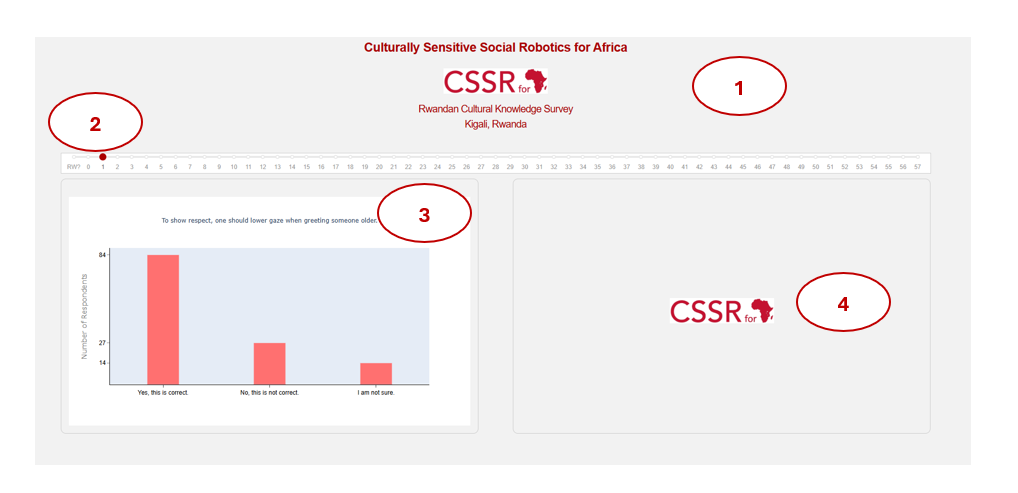
\includegraphics[width=\textwidth]{dashboard3.png} 
    \caption{CSSR4Africa Cultural Knowledge Survey Dashboard. The image illustrates the main sections: (1) Header Section, (2) Slider Section, (3) Bar Chart, and (4) Logo.}
    \label{fig:dashboard3}
\end{figure}

\begin{itemize}
    \item \textbf{(1) Header Section:} This section includes the title \textit{Culturally Sensitive Social Robotics for Africa}, the CSSR4Africa logo, and the location \textit{Kigali, Rwanda}. It serves as an introduction to the survey and its objectives.
    
    \item \textbf{(2) Slider Section:} Positioned below the header, the slider allows users to navigate through different survey questions, numbered from 0 to 57. Users can select a question, and the results update dynamically based on their selection. To move through all the questions, users can click on a specific question number on the slider or, after selecting the first question, use the keyboard arrow keys, a mouse, or a slide remote.
    
    \item \textbf{(3) Bar Chart:} This section presents the data visualization corresponding to the selected multiple-choice questions. The results are displayed using a bar graph, where the x-axis represents the different multiple-choice options available for the selected question, and the y-axis shows the count of responses for each choice. Based on these results, the option with the highest number of responses is chosen as the final conclusion for the survey question.
    
    \item \textbf{(4) Logo:} This section remains inactive since only multiple-choice questions without text have short answers.
\end{itemize}
%================================================================
The Figure \ref{fig:dashboard4} provides a visual representation of a multiple-choice question type that includes an ``Other" option, allowing respondents to specify their own answers in the dashboard layout.
\begin{figure}[H]
    \centering
    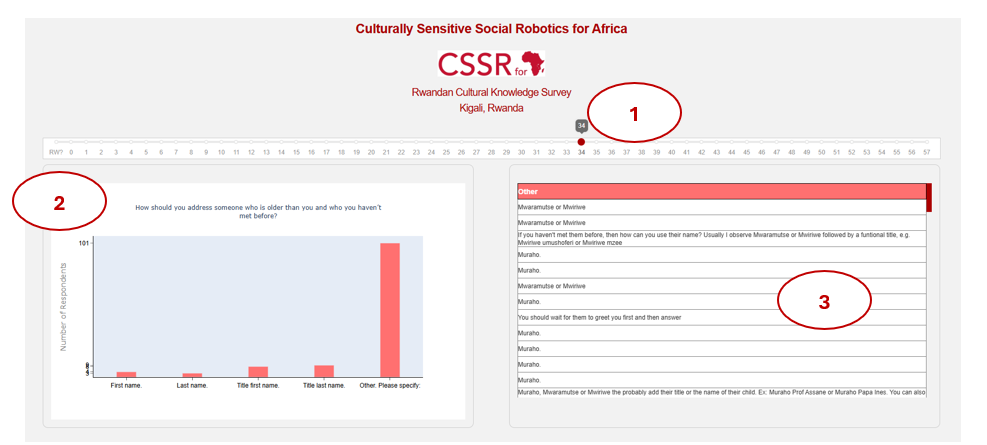
\includegraphics[width=\textwidth]{dashboard44.png} 
    \caption{CSSR4Africa Cultural Knowledge Survey Dashboard. The image illustrates the main sections: (1) Sample selected question using the slider, (2) Bar chart, and (3) Table displaying responses for the "Other" option.}
    \label{fig:dashboard4}
\end{figure}

\begin{itemize}
    \item \textbf{(1) Sample Selected Question:} This section represents a sample selected question that includes "Other" as a multiple-choice answer option.
    
    \item \textbf{(2) Bar Chart Visualization:} The bar chart visualization is similar to the one explained previously in Figure \ref{fig:dashboard3}.
    
    \item \textbf{(3) Table Display for "Other" Responses:} For respondents who select "Other" and provide their own answers, their responses are displayed in a table format, as shown in this section.
\end{itemize}
%================================================================
\newpage
\noindent The Figure \ref{fig:dashboard5} provides a visual representation of a multiple-choice question with a "Yes" or "No" option. If "Yes" is selected, respondents are allowed to specify their own answers, which are then displayed as tables in the dashboard layout.

\begin{figure}[H]
    \centering
    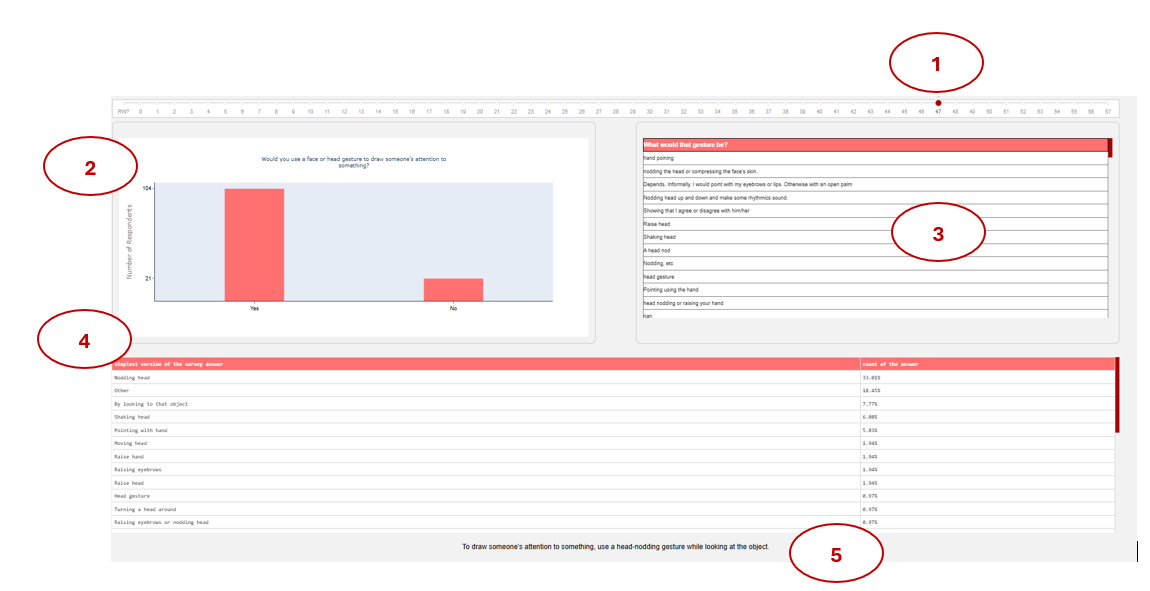
\includegraphics[width=\textwidth]{dashboard55.png} 
    \caption{CSSR4Africa Cultural Knowledge Survey Dashboard. The image illustrates the main sections: (1) Selected Question, (2) Multiple-Choice Responses, (3) Gesture Specification Table, (4) Annotated Gesture Table, and (5) Conclusion Answer.}
    \label{fig:dashboard5}
\end{figure}

\begin{itemize}
    \item \textbf{(1) Selected Question:} This section represents a randomly selected question that requires short answers, specifically requesting the gesture used for a particular type of behavior.
    
    \item \textbf{(2) Multiple-Choice Responses:} This section displays the responses for the multiple-choice question, illustrating whether gestures are used or not for the specified behavior.
    
    \item \textbf{(3) Gesture Specification Table:} If "Yes" is selected, respondents specify the gesture used, which is then displayed in the dashboard as a table.
    
    \item \textbf{(4) Annotated Gesture Table:} Before this table is generated, the table in section (3) is annotated to group similar gestures that were responded to using different phrases or expressions but belong to the same category. This section then organizes the gestures and displays the gesture names along with their corresponding percentage in the collected data.
    
    \item \textbf{(5) Conclusion Answer:} Based on the percentage shown in table (4), the final conclusion for the selected question is determined.
\end{itemize}
%================================================================
\newpage
\subsection*{File Structure}
The \texttt{dashboard} directory is organized to include data files, asset files, source code, a \texttt{README.md} file, requirements, and configuration files. The \texttt{config} folder contains essential configuration files, including \texttt{dashboard\_configuration.ini}, which uses key-value pairs to specify the data source—either an Excel file or a Google Spreadsheet. The \texttt{data} directory contains all survey-related datasets, such as \texttt{cssr-406009-380cb664c48a.json}, which serves as Google Sheets credentials for accessing survey data, and \texttt{Cultural Knowledge Survey.xlsx}, the primary Excel file containing survey responses. Additionally, the folder includes multiple CSV files categorized into hand, face, and body movement data. 
\\~\\
These files follow the naming format \texttt{<name>\_sdf\_<body|hand|face>\_<question number>} and represent the annotated versions of responses. These annotations help draw conclusions from short-answer questions, specifically from \texttt{Questions 47 to 57}, on the dashboard. 
\\~\\
The \texttt{src} folder contains the \texttt{assets} folder, which includes \texttt{dashboard\_style.css}, a stylesheet that defines the visual appearance of the dashboard, including layout, typography, tables, buttons, and interactive elements. Additionally, the folder includes \texttt{dashboard\_application.py}, which implements the Dash web application for visualizing survey responses with interactive features such as a question selection slider, bar chart visualizations, a dynamic data table, and an extra section that appears based on specific questions. The \texttt{dashboard\_implementation.py} script processes survey responses and updates visualizations dynamically. The \texttt{dashboard\_data\_processing.py} script loads and processes survey data from Google Sheets or an Excel file, filters Rwandan participants, categorizes survey questions, and prepares data for visualization. 
\\~\\
Lastly, \texttt{dashboard\_questions\_data.py} stores multiple-choice survey questions in a structured dictionary format, where each question is a key and answer choices are stored under "options", allowing for efficient bar graph generation and response categorization. Additionally, the \texttt{dashboard\_requirements.txt} file lists the dependencies required for running the application, and the \texttt{README.md} provides documentation on how to install, configure, and execute the dashboard. A detailed representation of the directory structure is shown in Figure \ref{fig:dashboard-dir}.
\\[1em] 
\begin{figure}[h]
\begin{center}
\begin{forest}
for tree={
  font=\small\ttfamily,
  grow'=0,
  child anchor=west,
  parent anchor=south,
  anchor=west,
  calign=first,
  inner sep=1pt,
  edge path={
    \noexpand\path [draw, \forestoption{edge}]
    (!u.south west) +(4pt,0) |- node[fill,inner sep=1pt] {} (.child anchor)\forestoption{edge label};
  },
  before typesetting nodes={
    if n=1
      {insert before={[,phantom]}}
      {}
  },
  fit=band,
  before computing xy={l=10pt},
}
[dashboard
  [config
    [dashboard\_configuration.ini]]
  [data]
    [cssr-406009-380cb664c48a.json]
    [Cultural Knowledge Survey.xlsx]
    [.]
    [.]
    [.]
  [src
    [\_\_pycache\_\_]
    [assets
      [dashboard\_style.css]]
    [dashboard\_application.py]
    [dashboard\_data\_processing.py]
    [dashboard\_implementation.py]
    [dashboard\_questions\_data.py]]
  [CSSR4AfricaLogo.svg]
  [dashboard\_requirements.txt]
  [README.md]]
\end{forest}
\end{center}
\caption{Directory structure for the CSSR4Africa Cultural Knowledge Survey Dashboard}
\label{fig:dashboard-dir}
\end{figure}


\newpage
%==============================================================
\subsection*{Executing the Dashboard}
To run the dashboard, first determine the data source: Google Sheets or an Excel file. During the active survey phase, Google Sheets was used to monitor real-time responses, as it dynamically updates when new data is received from the linked Google Form. Once survey collection is complete, the Google Sheet can be downloaded as an Excel file for further analysis in the dashboard. The dashboard supports both versions, and we can use the one that best suits the condition.

\subsubsection*{Getting Google Credentials (JSON File)}
Go to \href{https://console.cloud.google.com/}{Google Cloud Console} and sign in with your Google account. Create or select a project by clicking \href{https://console.cloud.google.com/}{Select a Project}, then enable the Google Sheets API via APIs \& \textbf{Services > Library}, search for Google Sheets API, and click\textbf{ Enable}; create credentials under APIs \& \textbf{Services > Credentials}, select Service Account, fill in details, assign at least Editor or Owner role, and click \textbf{Done}; generate and download the JSON key by navigating to the Keys tab, clicking \textbf{Add Key > Create New Key, choosing JSON}, and storing the file securely as credentials.json.
\newpage
\noindent
\textbf{Clone the Repository}
\begin{lstlisting}[style=linuxbashstyle]
git clone https://github.com/cssr4africa/cssr4africa.git
\end{lstlisting}
\begin{lstlisting}[style=linuxbashstyle]
cd dashboard
\end{lstlisting}
\textbf{Install Dependencies}
\begin{lstlisting}[style=linuxbashstyle]
pip install -r dashboard_requirements.txt
\end{lstlisting}
\textbf{Configure Data Source}\\[1em]
Modify the \textit{config/dashboard\_configuration.ini} file to specify the data source:\\[1em]
\textbf{Option 1:} Use Google Sheets: Set \texttt{use\_spreadsheet} to \texttt{true} and provide the \texttt{spreadsheet\_id} by adding the spreadsheet ID.
\begin{lstlisting}[style=linuxbashstyle]
        use_spreadsheet             true
        use_excel                   false
        spreadsheet_id              1nWPZX65-UQ-4nUGiKPIyPFY5AmtvW8ZdeyXEP-K5Vv
        excel_file                  Cultural Knowledge Survey.xlsx
        excel_sheet                 Sheet1_English_Version
        
\end{lstlisting}
%\newpage
\noindent \textbf{Option 2:} Use Excel File: Set \texttt{use\_excel} to \texttt{True} and \texttt{use\_spreadsheet} to \texttt{False}. Then, specify the file name in \texttt{excel\_file} and provide the sheet name. For example, if the first sheet of the Excel file is named "English," use that.
\begin{lstlisting}[style=linuxbashstyle]
        use_spreadsheet             false
        use_excel                   true
        spreadsheet_id              1nWPZX65-UQ-4nUGiKPIyPFY5AmtvW8ZdeyXEP-K5Vv
        excel_file                  Cultural Knowledge Survey.xlsx
        excel_sheet                 Sheet1_English_Version
\end{lstlisting}
 \textbf{Running the Dashboard}
\begin{lstlisting}[style=linuxbashstyle]
python .\src\dashboard_application.py
\end{lstlisting}
Click \href{http://127.0.0.1:8050/}{here} to open the dashboard.

\newpage
\bibliographystyle{unsrt}
%================================================================
\bibliography{cognitive_systems.bib}                                     % REPLACE with correct filename
\addcontentsline{toc}{section}{References}

 

\pagebreak
\section*{Principal Contributors}
%===============================================================
\label{contributors}
\addcontentsline{toc}{section}{Principal Contributors}
The main authors of this deliverable are as follows (in alphabetical order).
\blank
~
\blank
Eyerusalem Birhan, Carnegie Mellon University Africa.\\    
Muhirwa Richard, Carnegie Mellon University Africa.\\   
David Vernon, Carnegie Mellon University Africa.\\   


  

\newpage
\section*{Document History}
%================================================================
\addcontentsline{toc}{section}{Document History}
\label{document_history}

\begin{description}

\item [Version 1.0]~\\
First draft with survey questionnaire, for validation before conducting the survey. \\
David  Vernon. \\                       
25 October 2023.                                               


\item [Version 1.1]~\\
Fixed minor typos. \\
David  Vernon. \\                       
2 November 2023.      

\item [Version 1.2]~\\
Changed male/female to man/woman to determine the gender of the respondent. \\
Explained the context of the existing cultural knowledge.\\
Removed the question about name, to keep the survey anonymous.\\
Replaced question about being Rwandan by two questions on cultural heritage and nationality.\\
Removed the $<$ 20 age group.\\
David  Vernon. \\                       
20 November 2023.   

\item [Version 1.3]~\\
Changed the answers in Part 2 from I agree / do not agree to this is / is not correct.\\
David  Vernon. \\                       
20 November 2023.   

\item [Version 1.4]~\\
Removed several questions from Part 3 to align them with the CSSR4All questionnaire.\\
David  Vernon. \\                       
1 December 2023.   

\item [Version 1.5]~\\
Remove two questions from Part One. Group face, hand, and body gesture-related behaviors and minimize the number of questions from 48 to 30 for Part Three.\\
Eyerusalem Birhan. \\                       
19 January 2024.   

\item [Version 1.6]~
Added revision date to cover page.\\
Part 1, Q2: changed ``Woman" and ``Man" to ``Female" and ``Male".\\
Part 3, Q2: added ``Nod head" option.\\
Part 3, Q3: added ``Pass beside" option. \\
Part 3, Q7 - Q9: added ``Muraho" and ``Mwaramutse or Mwiriwe" options. \\
Part 3, Q21 - Q27: added ``head" to question. \\
Part 3, Q28: added ``hand" and ``body" to question.\\
Part 3, Q29 \& Q30: changed ``would you not use" to ``would you use" (to be consistent with other questions).\\
Removed References.\\
Added an appendix for a Kinyarwanda version of the questionnaire.\\
David  Vernon. \\                       
2 February 2024.   

\item [Version 1.7]~
Added content to appendix for the Kinyarwanda version of the questionnaire.\\
Eyerusalem Birhan.  \\                       
23 February 2024.   

\item [Version 1.8]~
Added links to the online questionnaire in Kinyarwanda and English.\\
David Vernon.  \\                       
31 July 2024.   

\item [Version 2.0]~
Added a section on the  knowledge  representation architecture suggested by Barbara Bruno et al. \cite{Brunoetal2019}.   Revised the Cultural knowledge ontology in Appendix III to align it more closely with the parameters of the robot actions, as suggested in \cite{Brunoetal2019}.  Added a section on mapping the questions in the survey to the ontology. Added a section on representing the knowledge derived from the questions in the survey using key-value pairs, with keys derived from the ontology. Added a provisional set of values for each key-value pair. Revised the abstract to reflect these changes. \\
David Vernon.  \\                       
19 August 2024.   

\item [Version 2.1]~
Added material on knowledge categories and knowledge representation. Removed lip and eyebrow gestures from  the ontology.  Moved the ontology from Appendix III to Fig. \ref{fig:knowledge_ontology}. \\        
David Vernon.\\               
22 August 2024.  

\item [Version 2.2]~ \\
Added Tables \ref{table:AllAnswers2} and \ref{table:AllAnswers3}, which contains the consensus answers to the fifty-seven questions in the survey. It includes the complete survey responses, except for questions 2-4, 2-5, and 2-8, which were rejected during the workshop, and question 3-28, which was excluded after observing the survey results. \\

Added Table~2, which contains the subset of the consensus answers to the 39 questions. These 39 questions were chosen based on Tables~3 and~4 by excluding questions marked with an asterisk that do not map to any of the ontology keys.\\

Updated Table~5. Added values under the Values column which were previously empty and updated the key values as follows:
\begin{itemize}
    \item Replaced PassingPosition with two new key values: PassingPositionAvoid and PassingPositionPreferred.
    
    \item Replaced AccompanyingDistance with two new key values: AccompanyingDistanceAvoid and AccompanyingDistancePreferred.
    
    \item Added a new key: WordAddressMethod.
    
    \item Replaced TurnTakingUtterance with three new key values: TurnTakingUtteranceSignal, TurnTakingUtteranceAvoid, and TurnTakingUtteranceInitiates.
    
    \item Replaced FocusofAttentionTarget with three new key values: FocusofAttentionTargetGreetingOlder, FocusofAttentionTargetAddressed, and FocusofAttentionTargetExplanation.

    \item Replaced EyeContactDuration with EyeContactDurationInteraction.
    
    \item Replaced EyeContactFrequency with six new key 
 EyeContactFrequencyExplainOlder, EyeContactFrequencyExplainYounger, EyeContactFrequencyListen, EyeContactFrequencyListenOlder, and EyeContactFrequencyListenYounger.
 
    \item Replaced NodExtent with eight new key values: 
    NodExtentAttention, BowExtentGratitude, NodExtentAgreement, BowExtentRespect, FacialGestureFriendliness, FacialGestureConfusion, NodExtentComprehension and NodExtentListening.
    
     \item Replaced DeicticShape with two new key values: 
    DeicticShapePoint and DeicticShapePointAvoid.
    
    \item Replaced IconicShape with IconicShapeSpeaking.
    
    \item Replaced SymbolicShape with nine new key values: 
    SymbolicShapeRespect, SymbolicShapeRespectHandShake, SymbolicShapeGratitude, SymbolicShapeAgreement, SymbolicShapeFriendliness, SymbolicShapeConfusion, SymbolicShapeComprehension, SymbolicShapeAvoid and SymbolicShapeAvoidGreeting.
    
     \item Replaced BowExtent with three new key values: BowExtentGreeting, BowExtentGratitude and BowExtentRespect.
     \item Added a new key: IconicShapeSpeaking.
\end{itemize}
Eyerusalem Birhan.\\
28 November 2024.   


\item [Version 2.3]~ \\
Moved Section 2 Representation of Cultural Knowledge, and Section 3.2 Action and Cultural Parameter Values to Deliverable D5.4.1.\\
David Vernon.\\
21 December 2024.   

\item [Version 2.4]~ \\
Added the summary of the survey questions in Tables \ref{table:questions2} and \ref{table:questions3}. \\
Added Section  \ref{section:methodology} Survey Methodology. \\
David Vernon.\\
29 December 2024. 


\item [Version 2.5]~ \\
Added Appendix III: Dashboard for Cultural Knowledge Survey Questionnaire Responses (\ref{section: appendixiii}), which explains the dashboard in detail and how to execute it.\\
Eyerusalem Birhan.\\
21 February 2025. 

\item [Version 2.6]~ \\
Update the slider explanation, the file structure, and the executing the dashboard sections. \\
Eyerusalem Birhan.\\
16 March 2025. 

\newpage

\item [Version 3.0]~ \\
Fixed formatting problems caused by using geometry and lmodern packages: incorrect margins and incorrect fonts on cover page, respectively. \\
Responsible person changed to Eyerusalem Birhan to better reflect the time and effort spent on the deliverable.\\
David Vernon.\\
29 April 2025. 

\item [Version 3.1]~ \\
Resolved references\\
David Vernon.\\
16 June 2025. 

\end{description}

\end{document}

